\documentclass[12pt,letterpaper]{article}
\usepackage[utf8]{inputenc}
\usepackage[spanish]{babel}
\usepackage{amsmath}
\usepackage{color}
\usepackage{subcaption}
\usepackage{amsfonts}
\usepackage{hyperref}
 \hypersetup{
     colorlinks=true,
     linkcolor=blue,
     filecolor=blue,
     citecolor = blue,      
     urlcolor=cyan,
     }
\usepackage{amssymb}
\usepackage{listings}
\usepackage{graphicx}
\usepackage[left=2cm,right=2cm,top=2cm,bottom=1.8cm]{geometry}
\setlength{\parskip}{5mm}

\title{\textsc{Práctica 3: \\Teoría de colas}}
\author{\textsc{Fabiola Vázquez}}

\setlength{\parindent}{0cm}
\renewcommand{\lstlistingname}{Código}
\begin{document}
\maketitle
\hrule
\section{Experimento}
El objetivo de esta práctica \cite{elisap3} es examinar si los tiempos de ejecución de la \textit{tarea} son afectados por los diversos ordenamientos de un vector (ascendente, descendente, pseudoaleatorio, primero los primos, al final los primos) o por las variaciones  de los núcleos que se asignan al cluster. Dicho vector, que contiene números primos extraídos de \url{https://primes.utm.edu/lists/small/millions/}, contiene el 50\% de números primos. También, se analiza si la proporción de primos en el vector afecta los tiempos de ejecución. En cada experimento se realizan 50 réplicas. Dicho experimento se realiza con el software R versión 3.7.9 \cite{R} en un cuaderno de Jupyter \cite{jupyter}.

En la primera parte del experimento, se considera como \textit{tarea} determinar si un número es primo, para ello se utiliza la función descrita en el código \ref{lst:gc1}, elaborado por la Dra. Elisa Schaeffer \cite{elisa}.
\begin{lstlisting}[label=lst:gc1,caption=Función para determinar si un número es primo., frame = single]
primo <- function(n){
    if (n == 1 || n == 2) {
        return(TRUE)
    }
    if (n%%  2 == 0) {
        return(FALSE)
    }
    for (i in seq(3, max(3, ceiling(sqrt(n))), 2)) {
        if ((n%%  i) == 0) {
            return(FALSE)
        }
    }
    return(TRUE)
}
\end{lstlisting} 
En la figura \ref{primos} se muestran gráficos de caja en donde se tienen los tiempos de cada uno de los cinco órdenes del vector variando los núcleos. Como se puede apreciar en dicha figura, no parece haber gran diferencia entre los tiempos de ejecución al variar los núcleos utilizados.

Realizamos una prueba de Kruskal-Wallis para verificar si los núcleos o el tipo de orden del vector afectan los tiempos de ejecución. En el cuadro \ref{datos1} se tienen los valores $p$ obtenidos con dicha prueba, con lo que se concluye que la cantidad de núcleos no afecta los tiempos de ejecución y los órdenes del vector sí afectan.
\begin{table}
\centering
\caption{Valores $p$ obtenidos de la prueba de Kruskal-Wallis en el primer experimento.}
\begin{tabular}{|c|c|}
\hline 
Datos & valor $p$ \\ 
\hline 
Tiempo $\sim$ Núcleo & 0.0076 \\ 
\hline 
Tiempo $\sim$ Orden & 0.4490 \\ 
\hline 
\end{tabular} 
\label{datos1}
\end{table}
\begin{figure}
 	\centering
 	\begin{subfigure}[b]{0.45\linewidth}
 		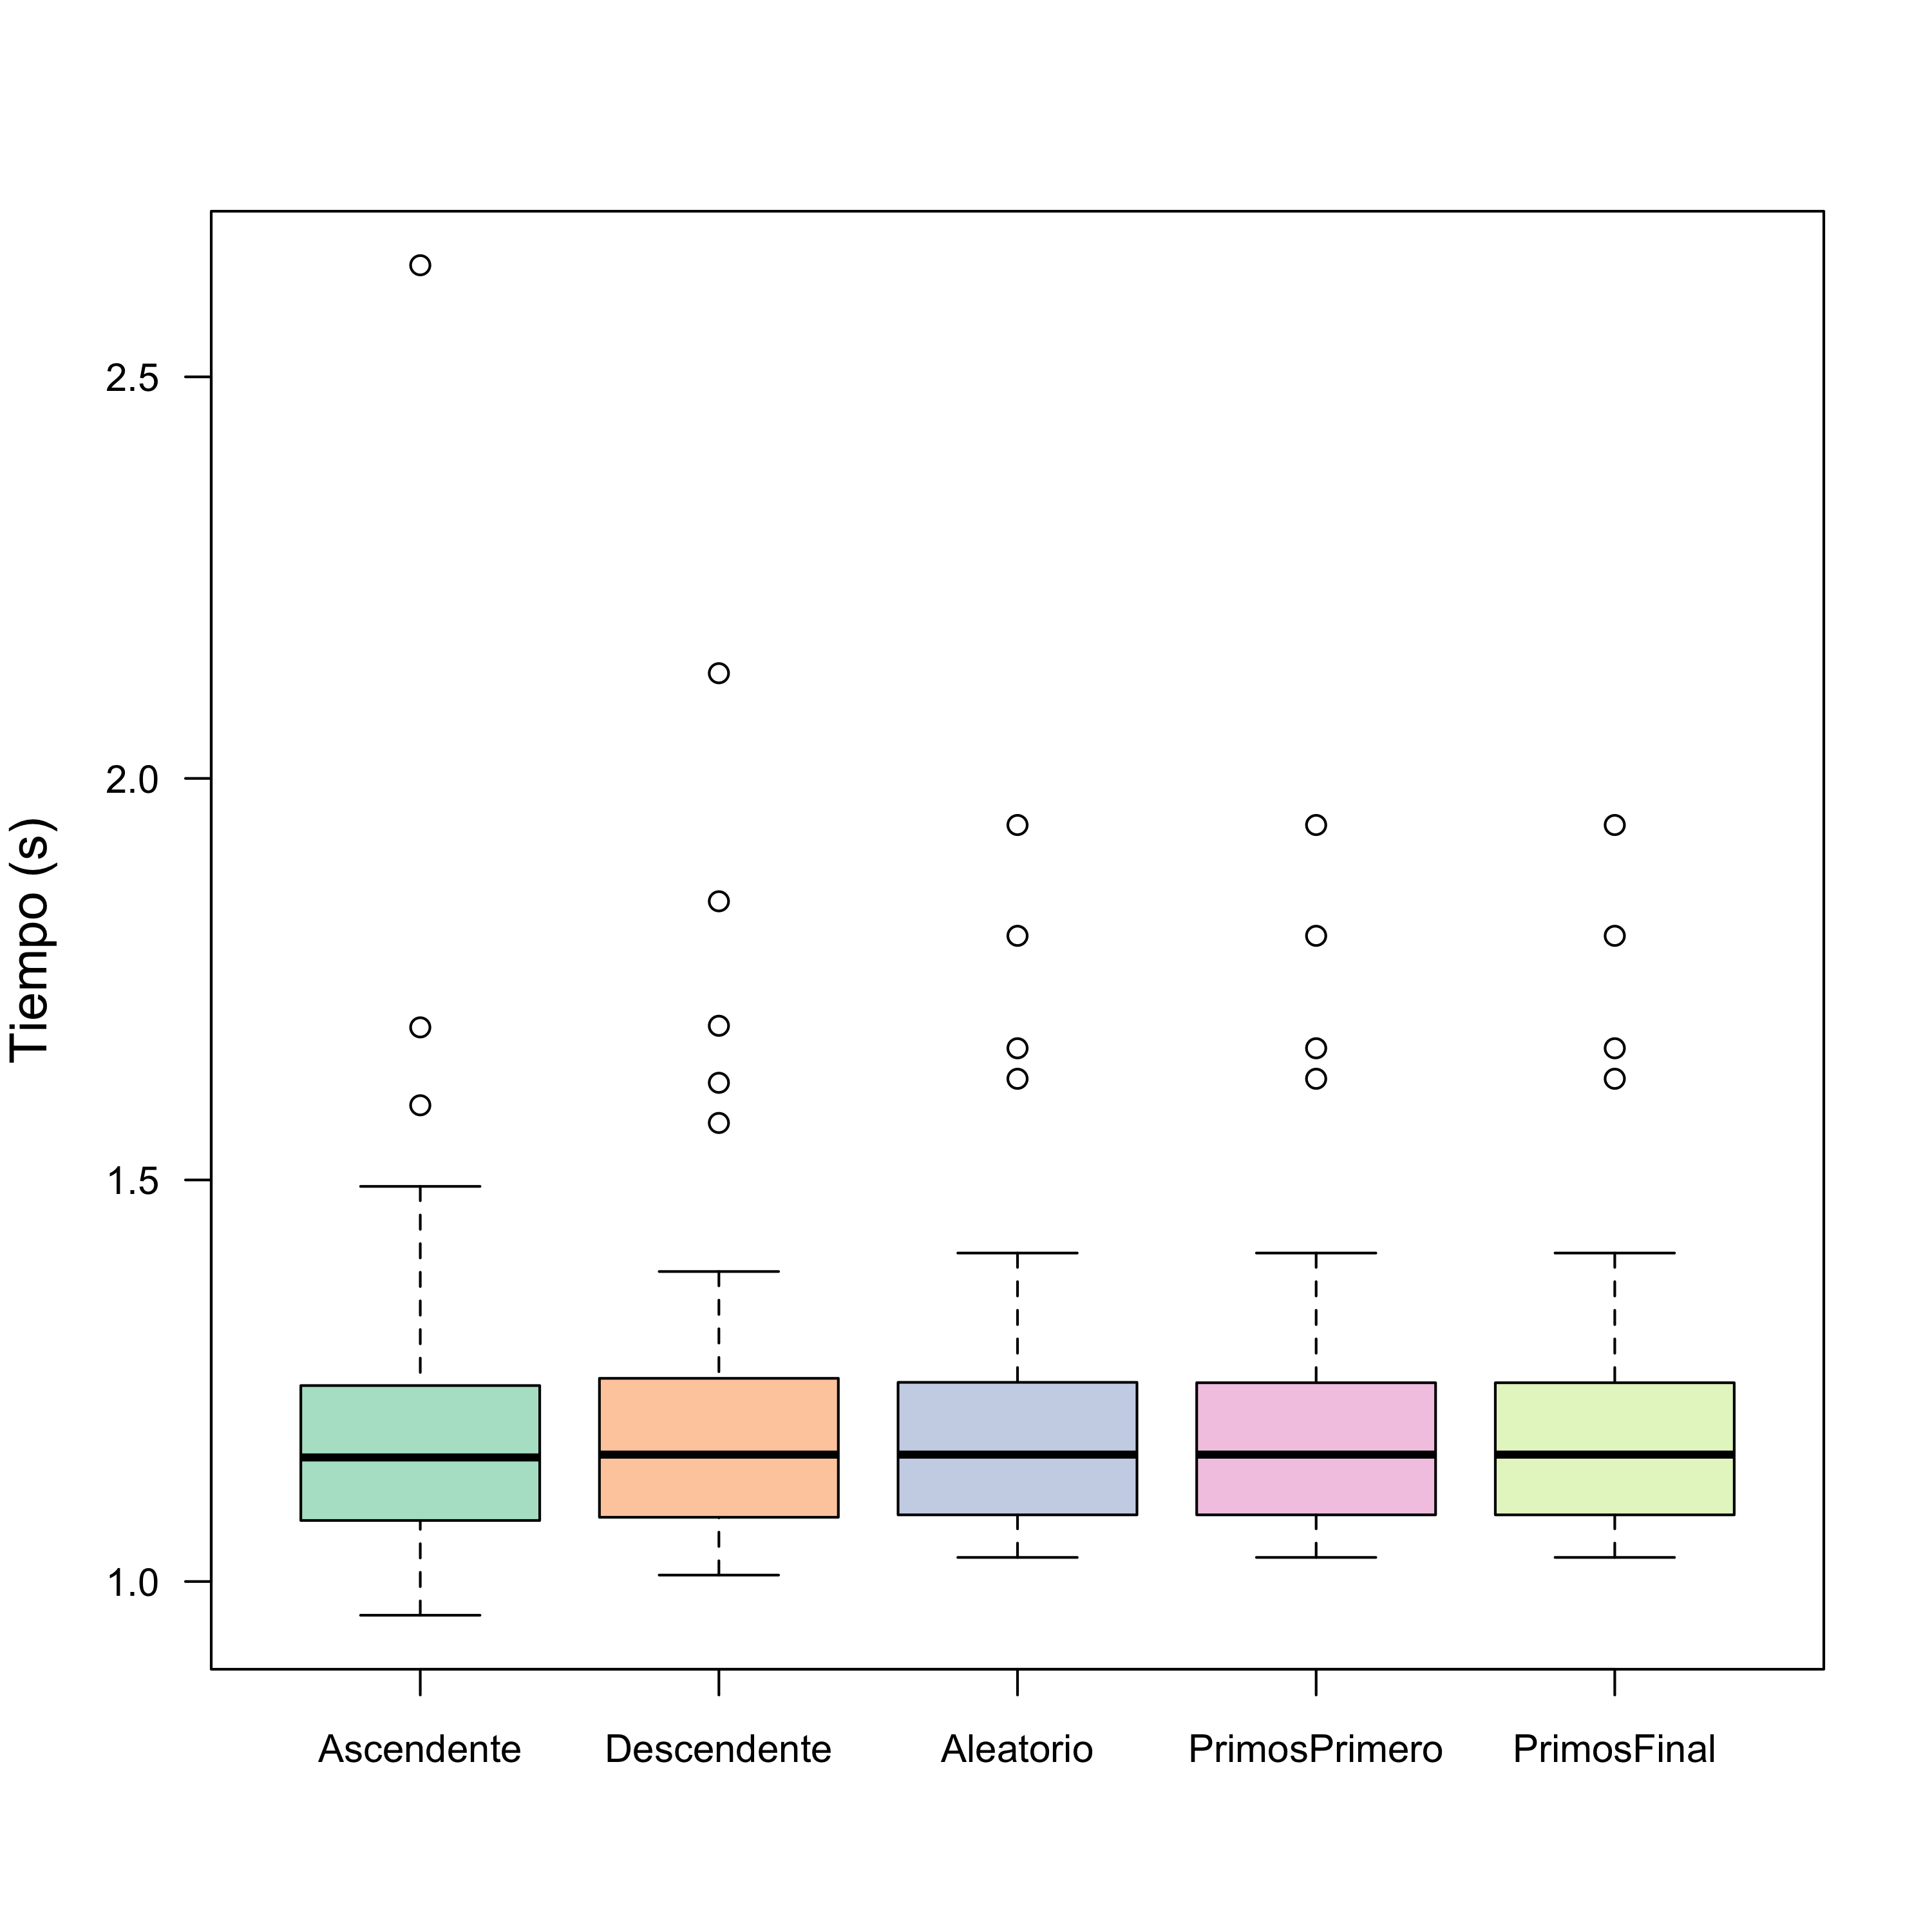
\includegraphics[width=\linewidth]{primos_1.png}
 		 \caption{Usando tres núcleos.}
 		\label{primos3}
 	\end{subfigure}
 	\begin{subfigure}[b]{0.45\linewidth}
 		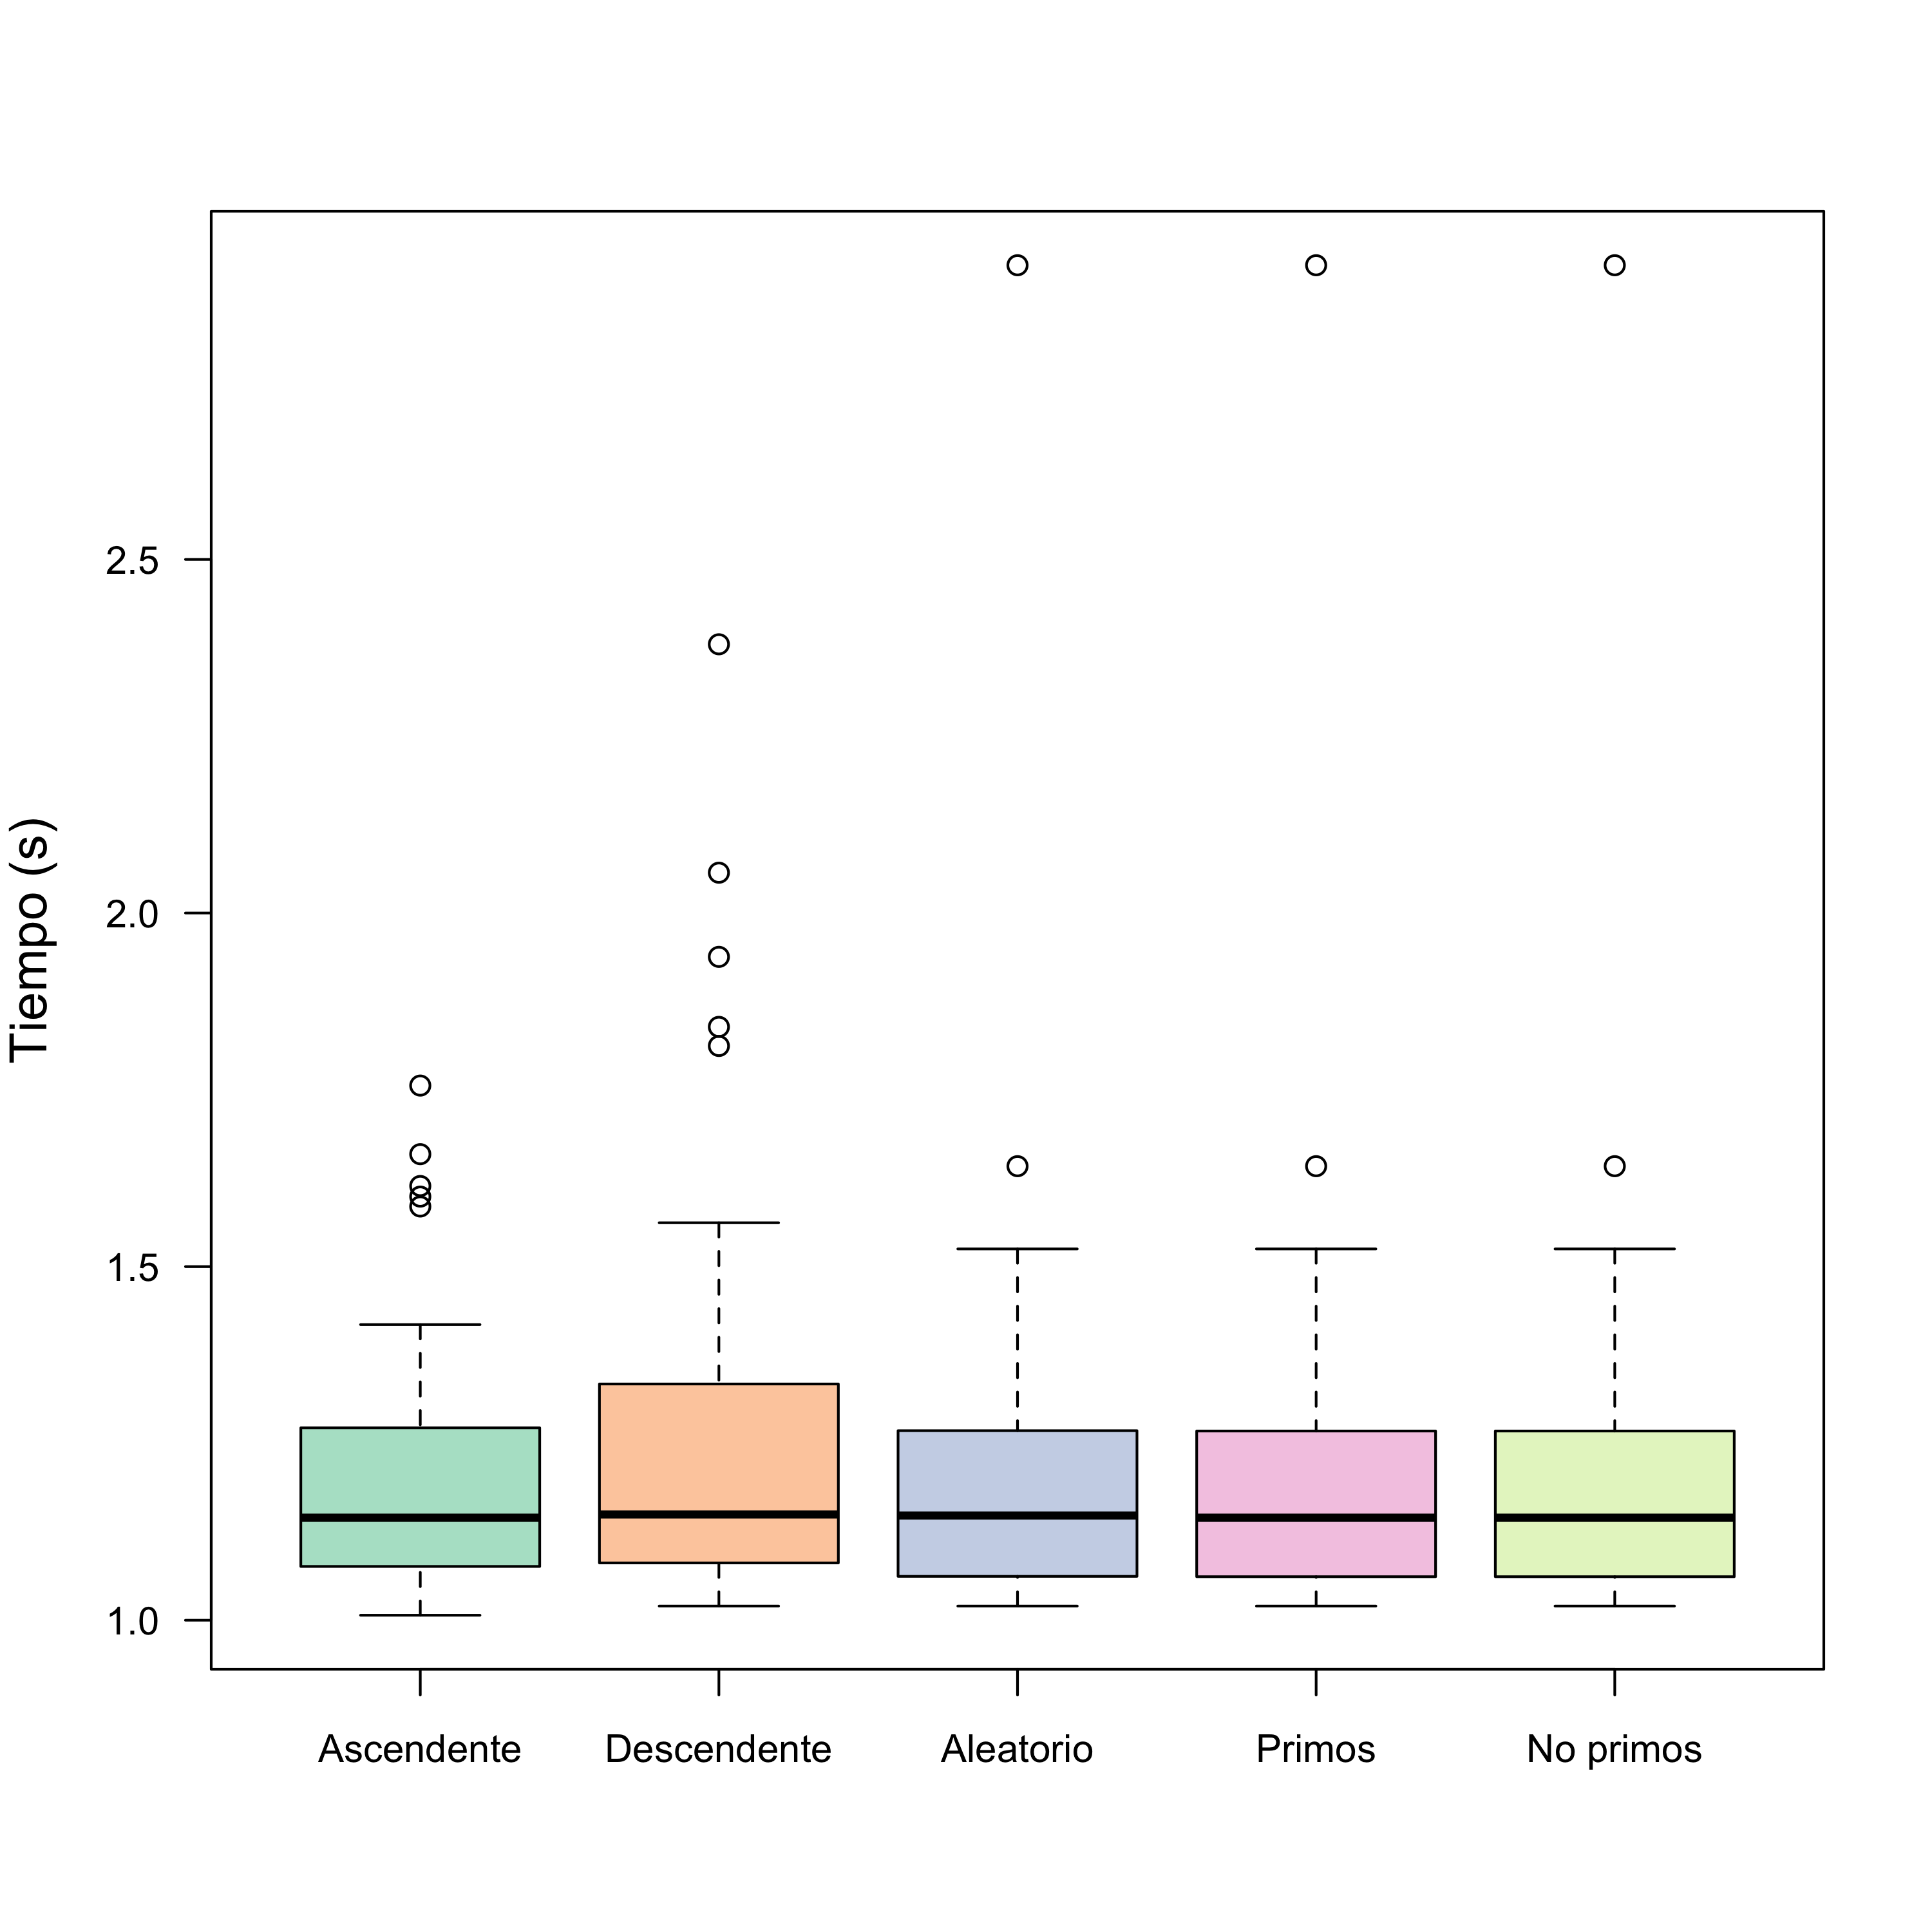
\includegraphics[width=\linewidth]{primos_2.png}
 		 \caption{Usando dos núcleos.}
 		\label{primos2}
 	\end{subfigure}
 	\begin{subfigure}[b]{0.45\linewidth}
 		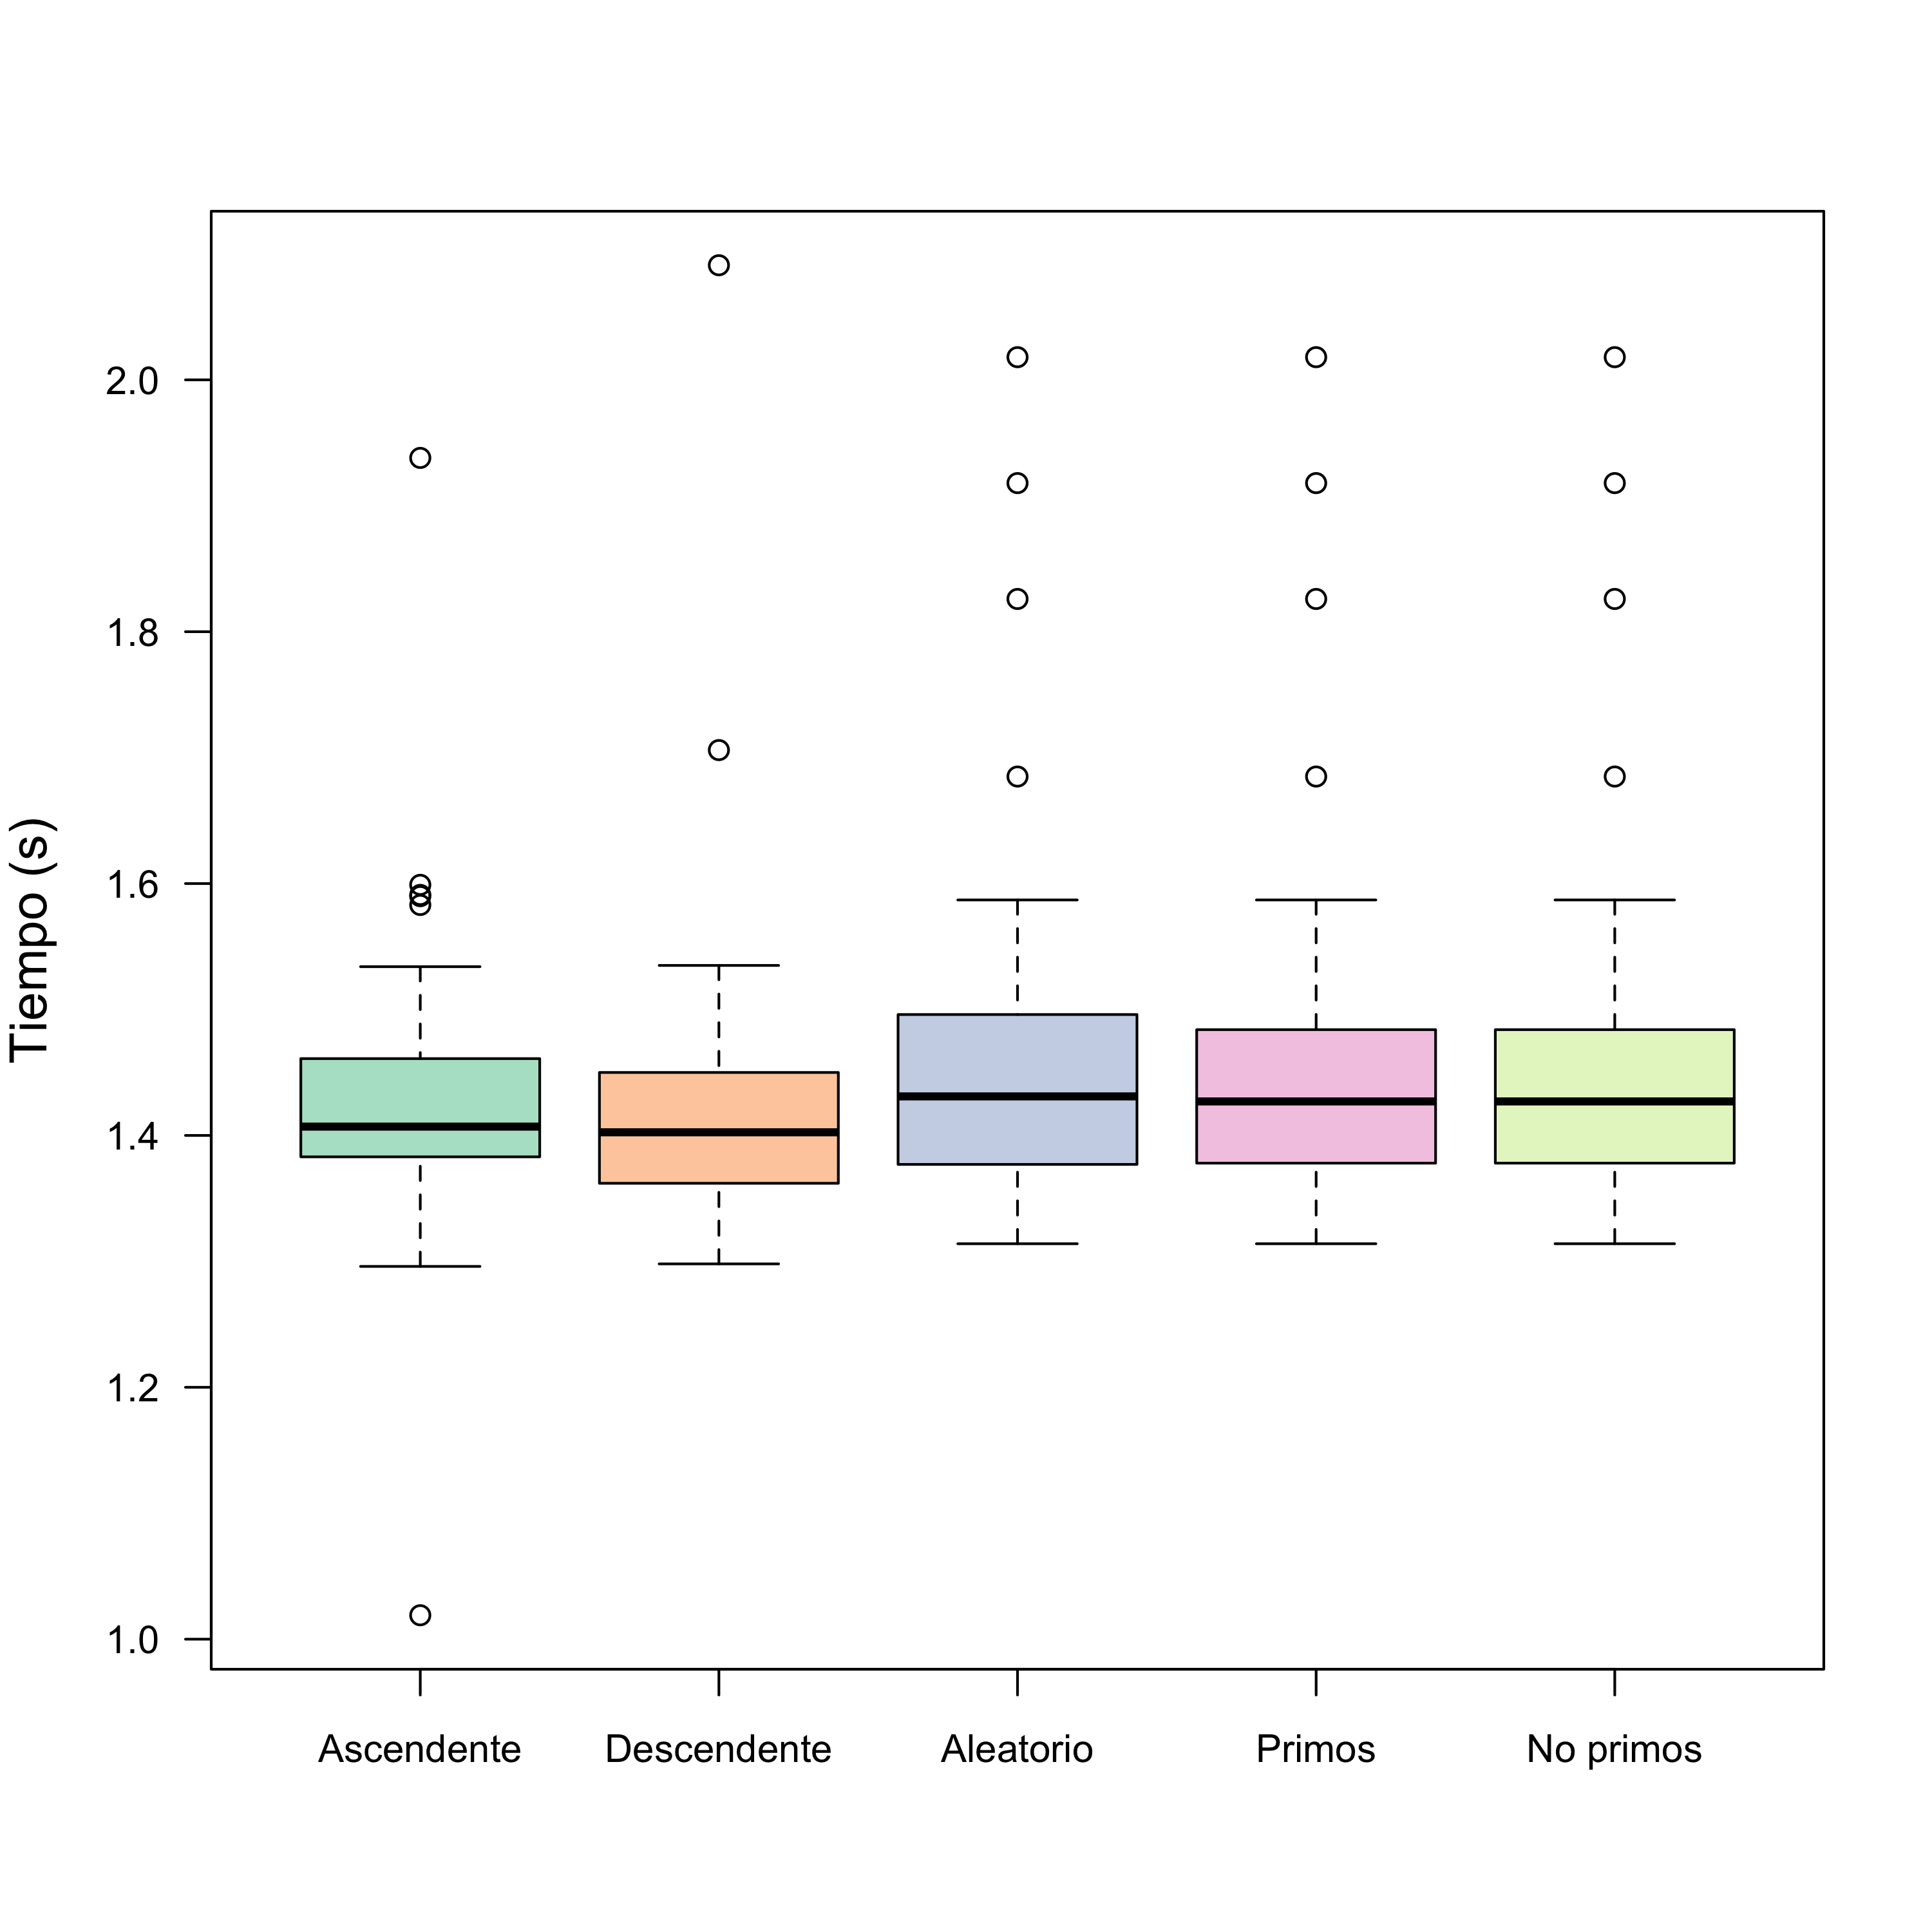
\includegraphics[width=\linewidth]{primos_3.png}
 		\caption{Usando un núcleo.}
 		\label{primos1}
 	\end{subfigure}
 	\caption{Gráfica de cajas variando los núcleos usados en el experimento.}  		
\label{primos}
 \end{figure}

Ahora, se analiza el efecto que tiene, en los tiempos de ejecución, la proporción de números primos que hay en el vector. Para ello, crearemos un vector variando el porcentaje de primos, de 0\% a 100\% en incrementos de 10\%. En la figura \ref{porcentaje} tenemos gráficas de caja con los tiempos de ejecución variando la cantidad de núcleos usados. Se nota que entre mayor proporción de primos, mayor es el tiempo de ejecución. 

Se realiza, también, una prueba de Kruskal-Wallis para comprobar dicha suposición. En el cuadro \ref{datos2} se tienen los valores $p$ obtenidos en la prueba, con lo cuál, se concluye que el porcentaje de primos que hay en el vector afecta el tiempo de ejecución de la tarea. 

\begin{table}
\centering
\caption{Valores $p$ obtenidos de la prueba de Kruskal-Wallis en el experimento de variación del porcentaje de primos en el vector.}
\begin{tabular}{|c|c|}
\hline 
Datos & valor $p$ \\ 
\hline 
Tiempo $\sim$ Núcleo & 0.0016 \\ 
\hline 
Tiempo $\sim$ Porcentaje de Primos & 0.2926\\ 
\hline 
\end{tabular} 
\label{datos2}
\end{table}
\begin{figure}
 	\centering
 	\begin{subfigure}[b]{0.45\linewidth}
 		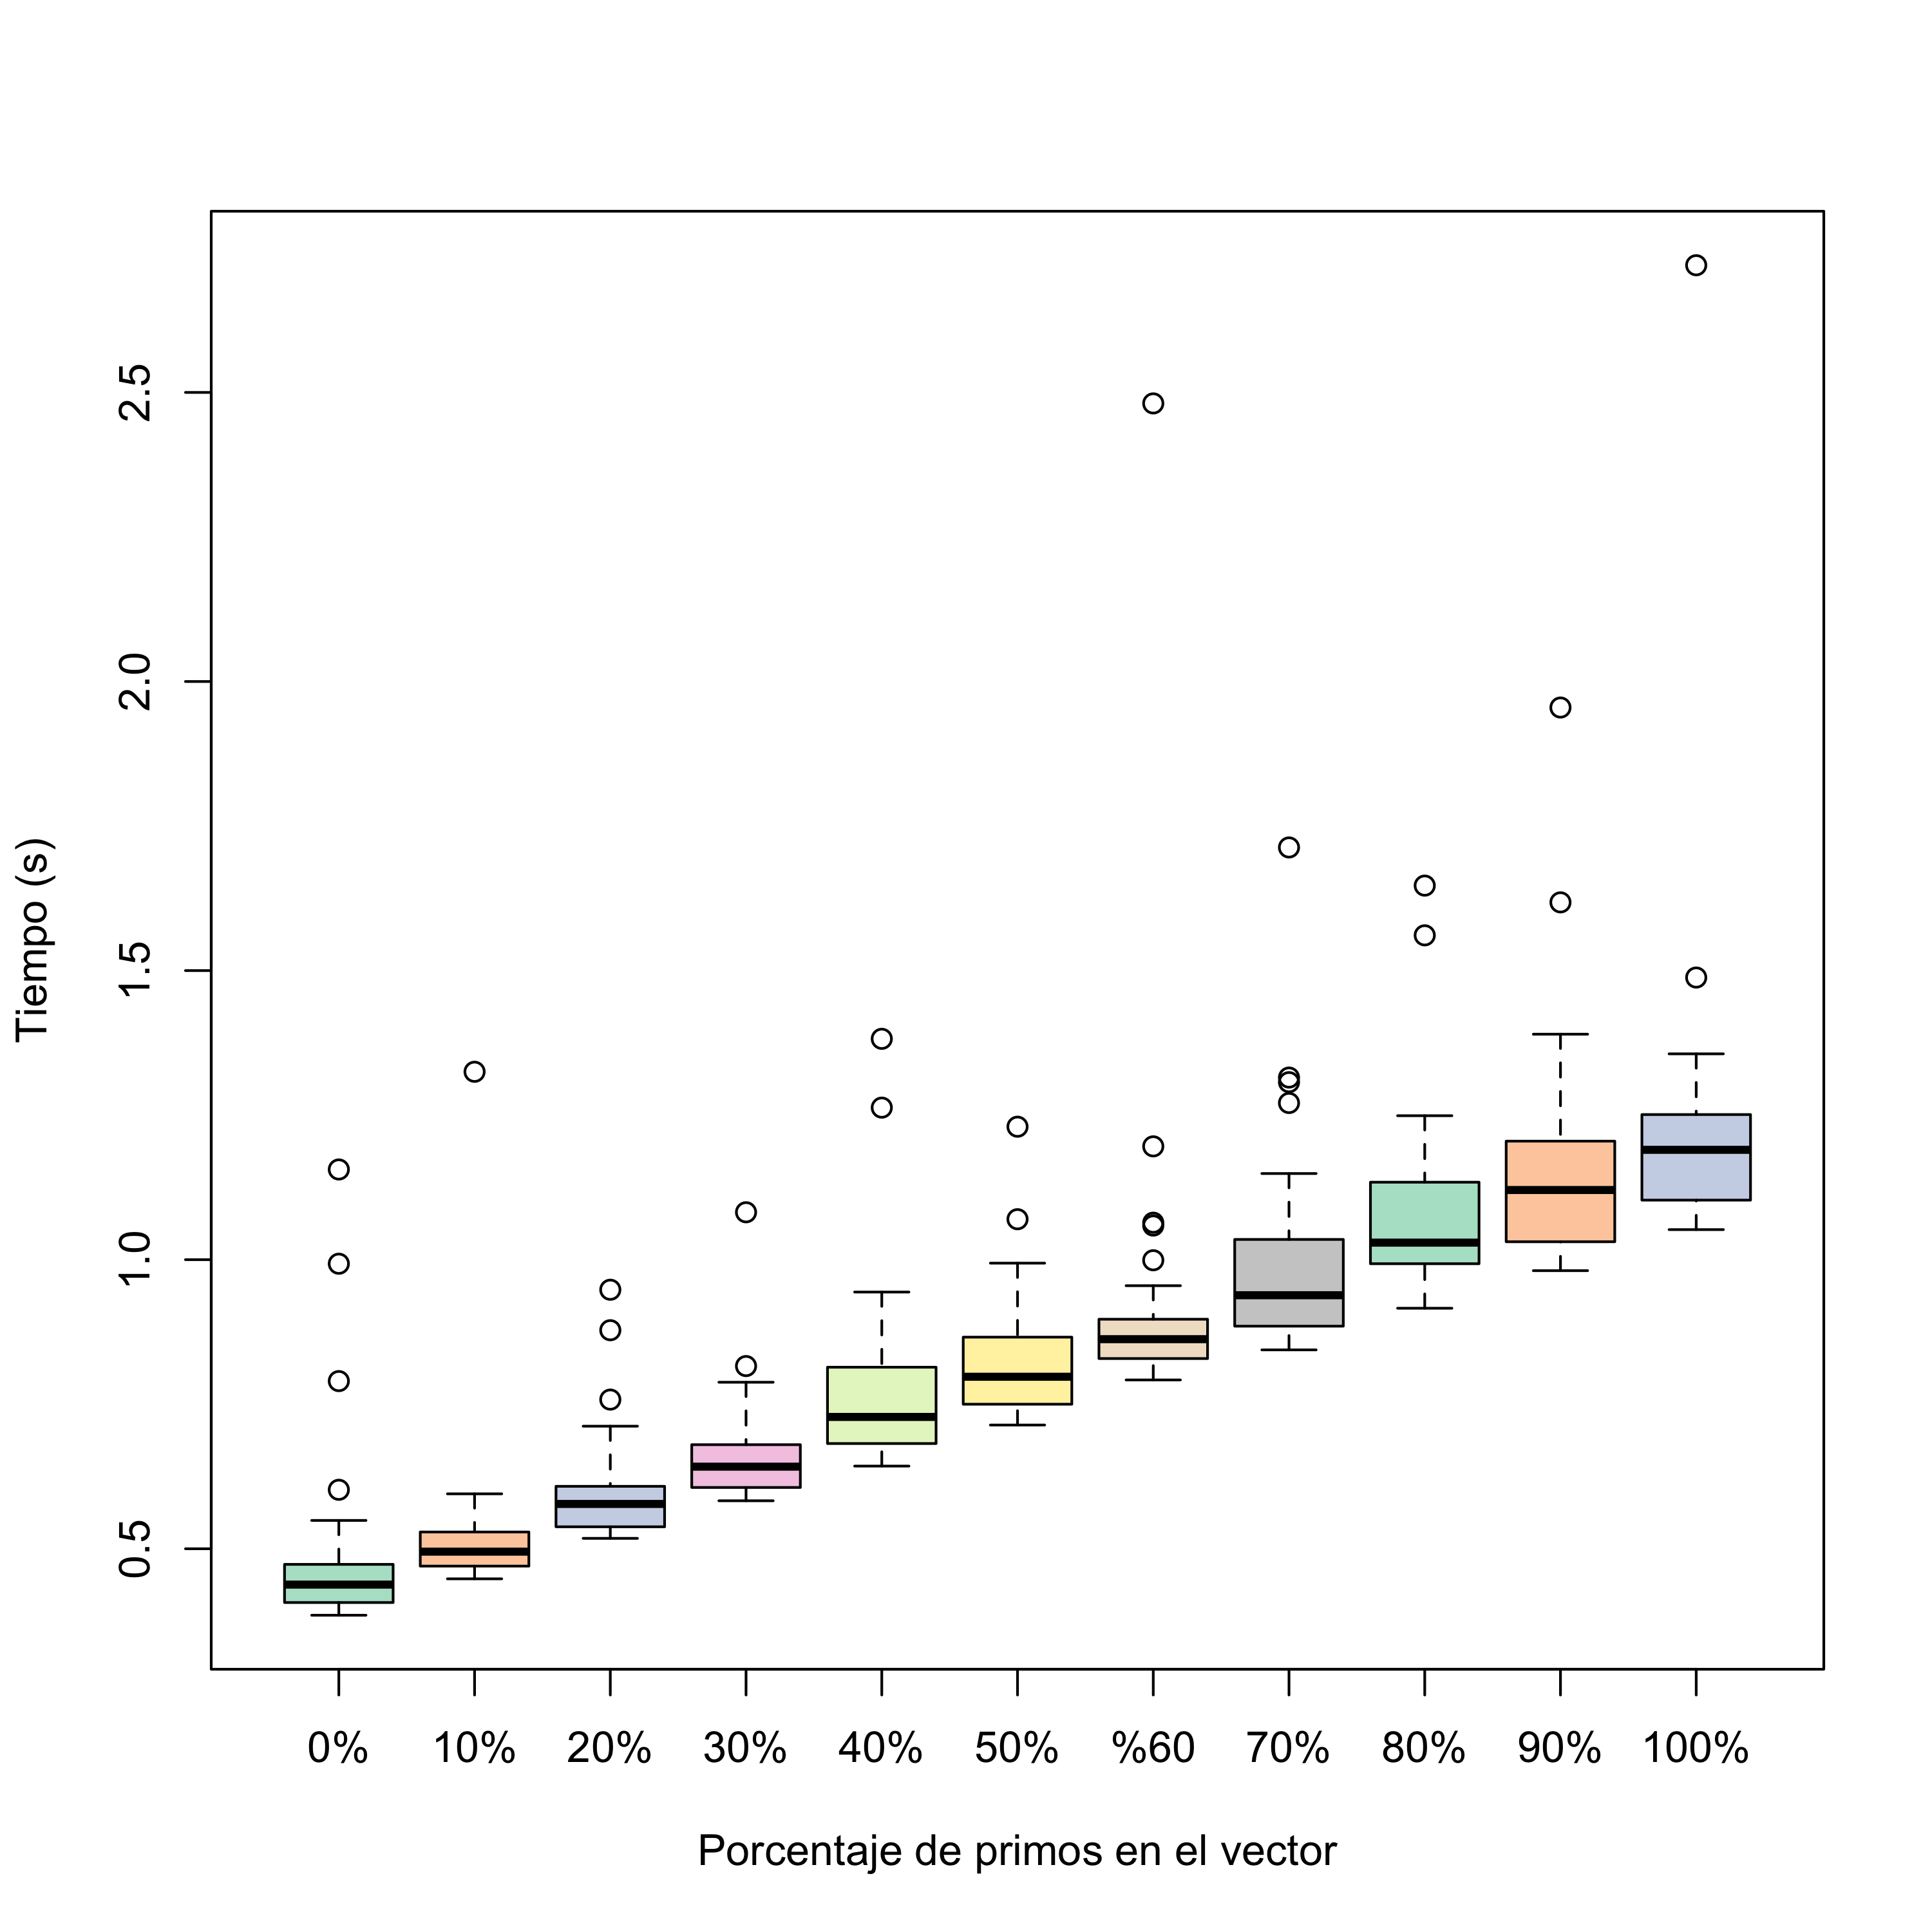
\includegraphics[width=\linewidth]{porcentaje_1.png}
 		 \caption{Usando tres núcleos.}
 		\label{porcentaje3}
 	\end{subfigure}
 	\begin{subfigure}[b]{0.45\linewidth}
 		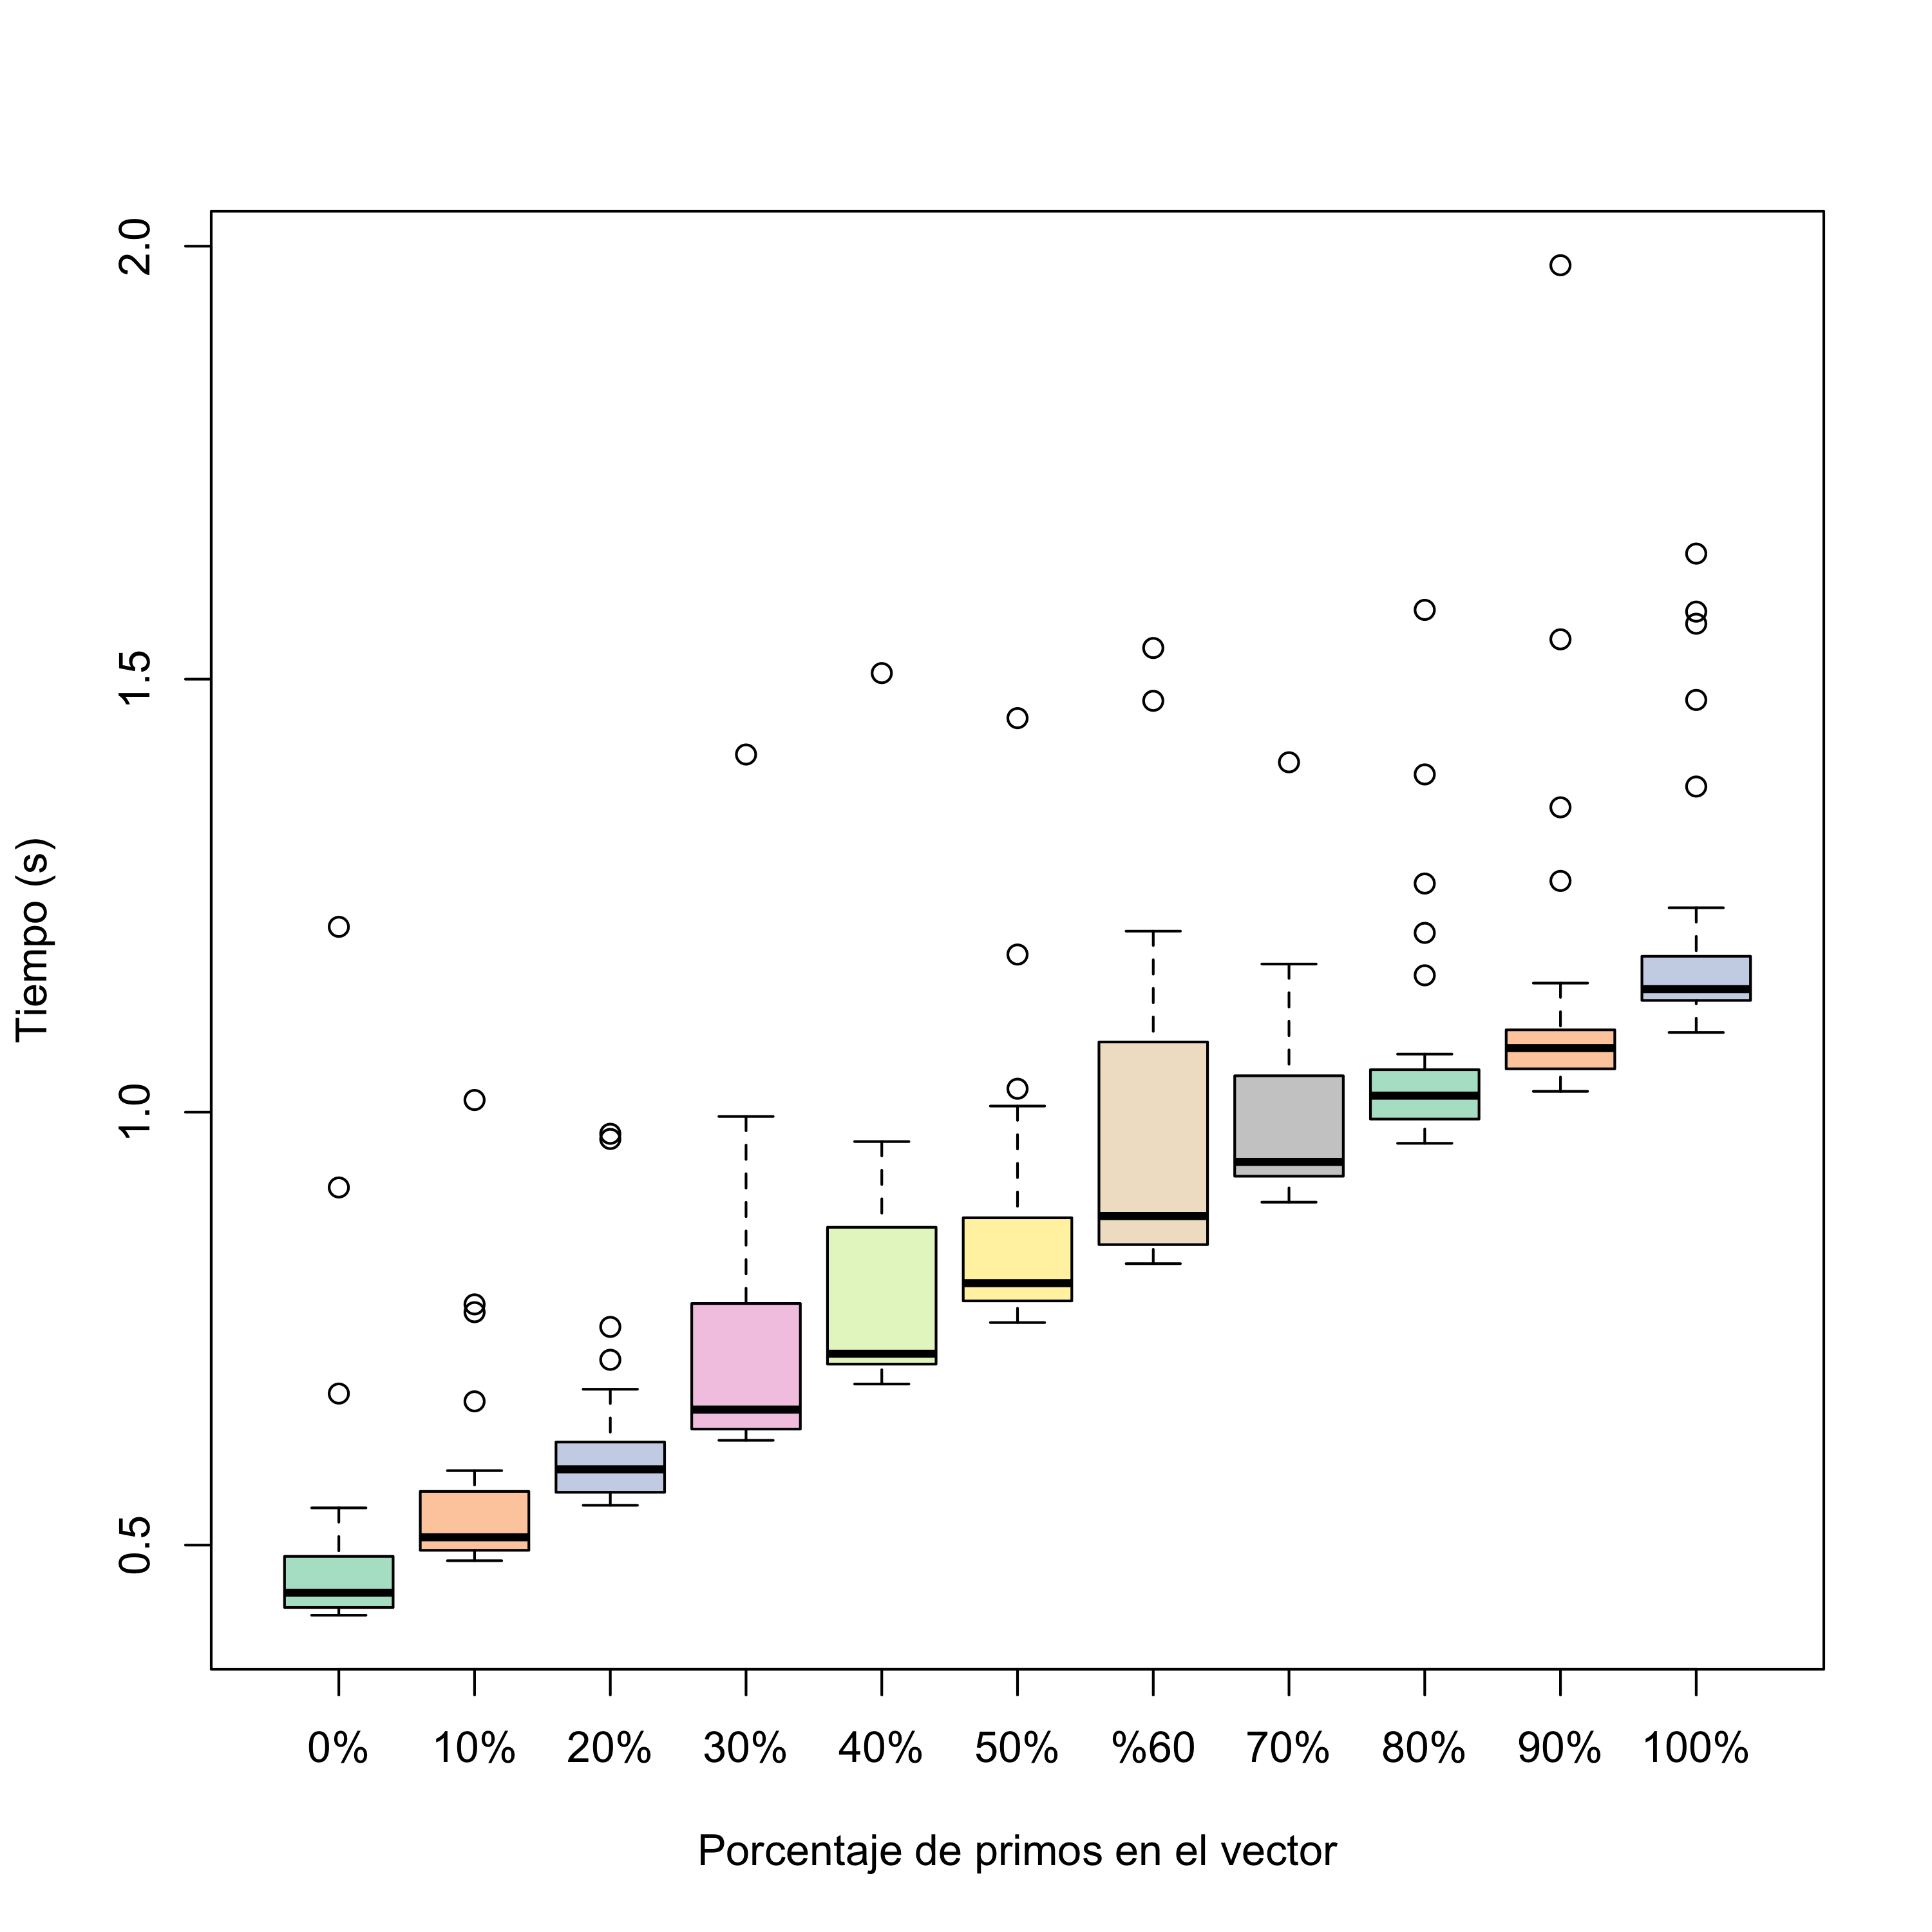
\includegraphics[width=\linewidth]{porcentaje_2.png}
 		 \caption{Usando dos núcleos.}
 		\label{porcentaje2}
 	\end{subfigure}
 	\begin{subfigure}[b]{0.45\linewidth}
 		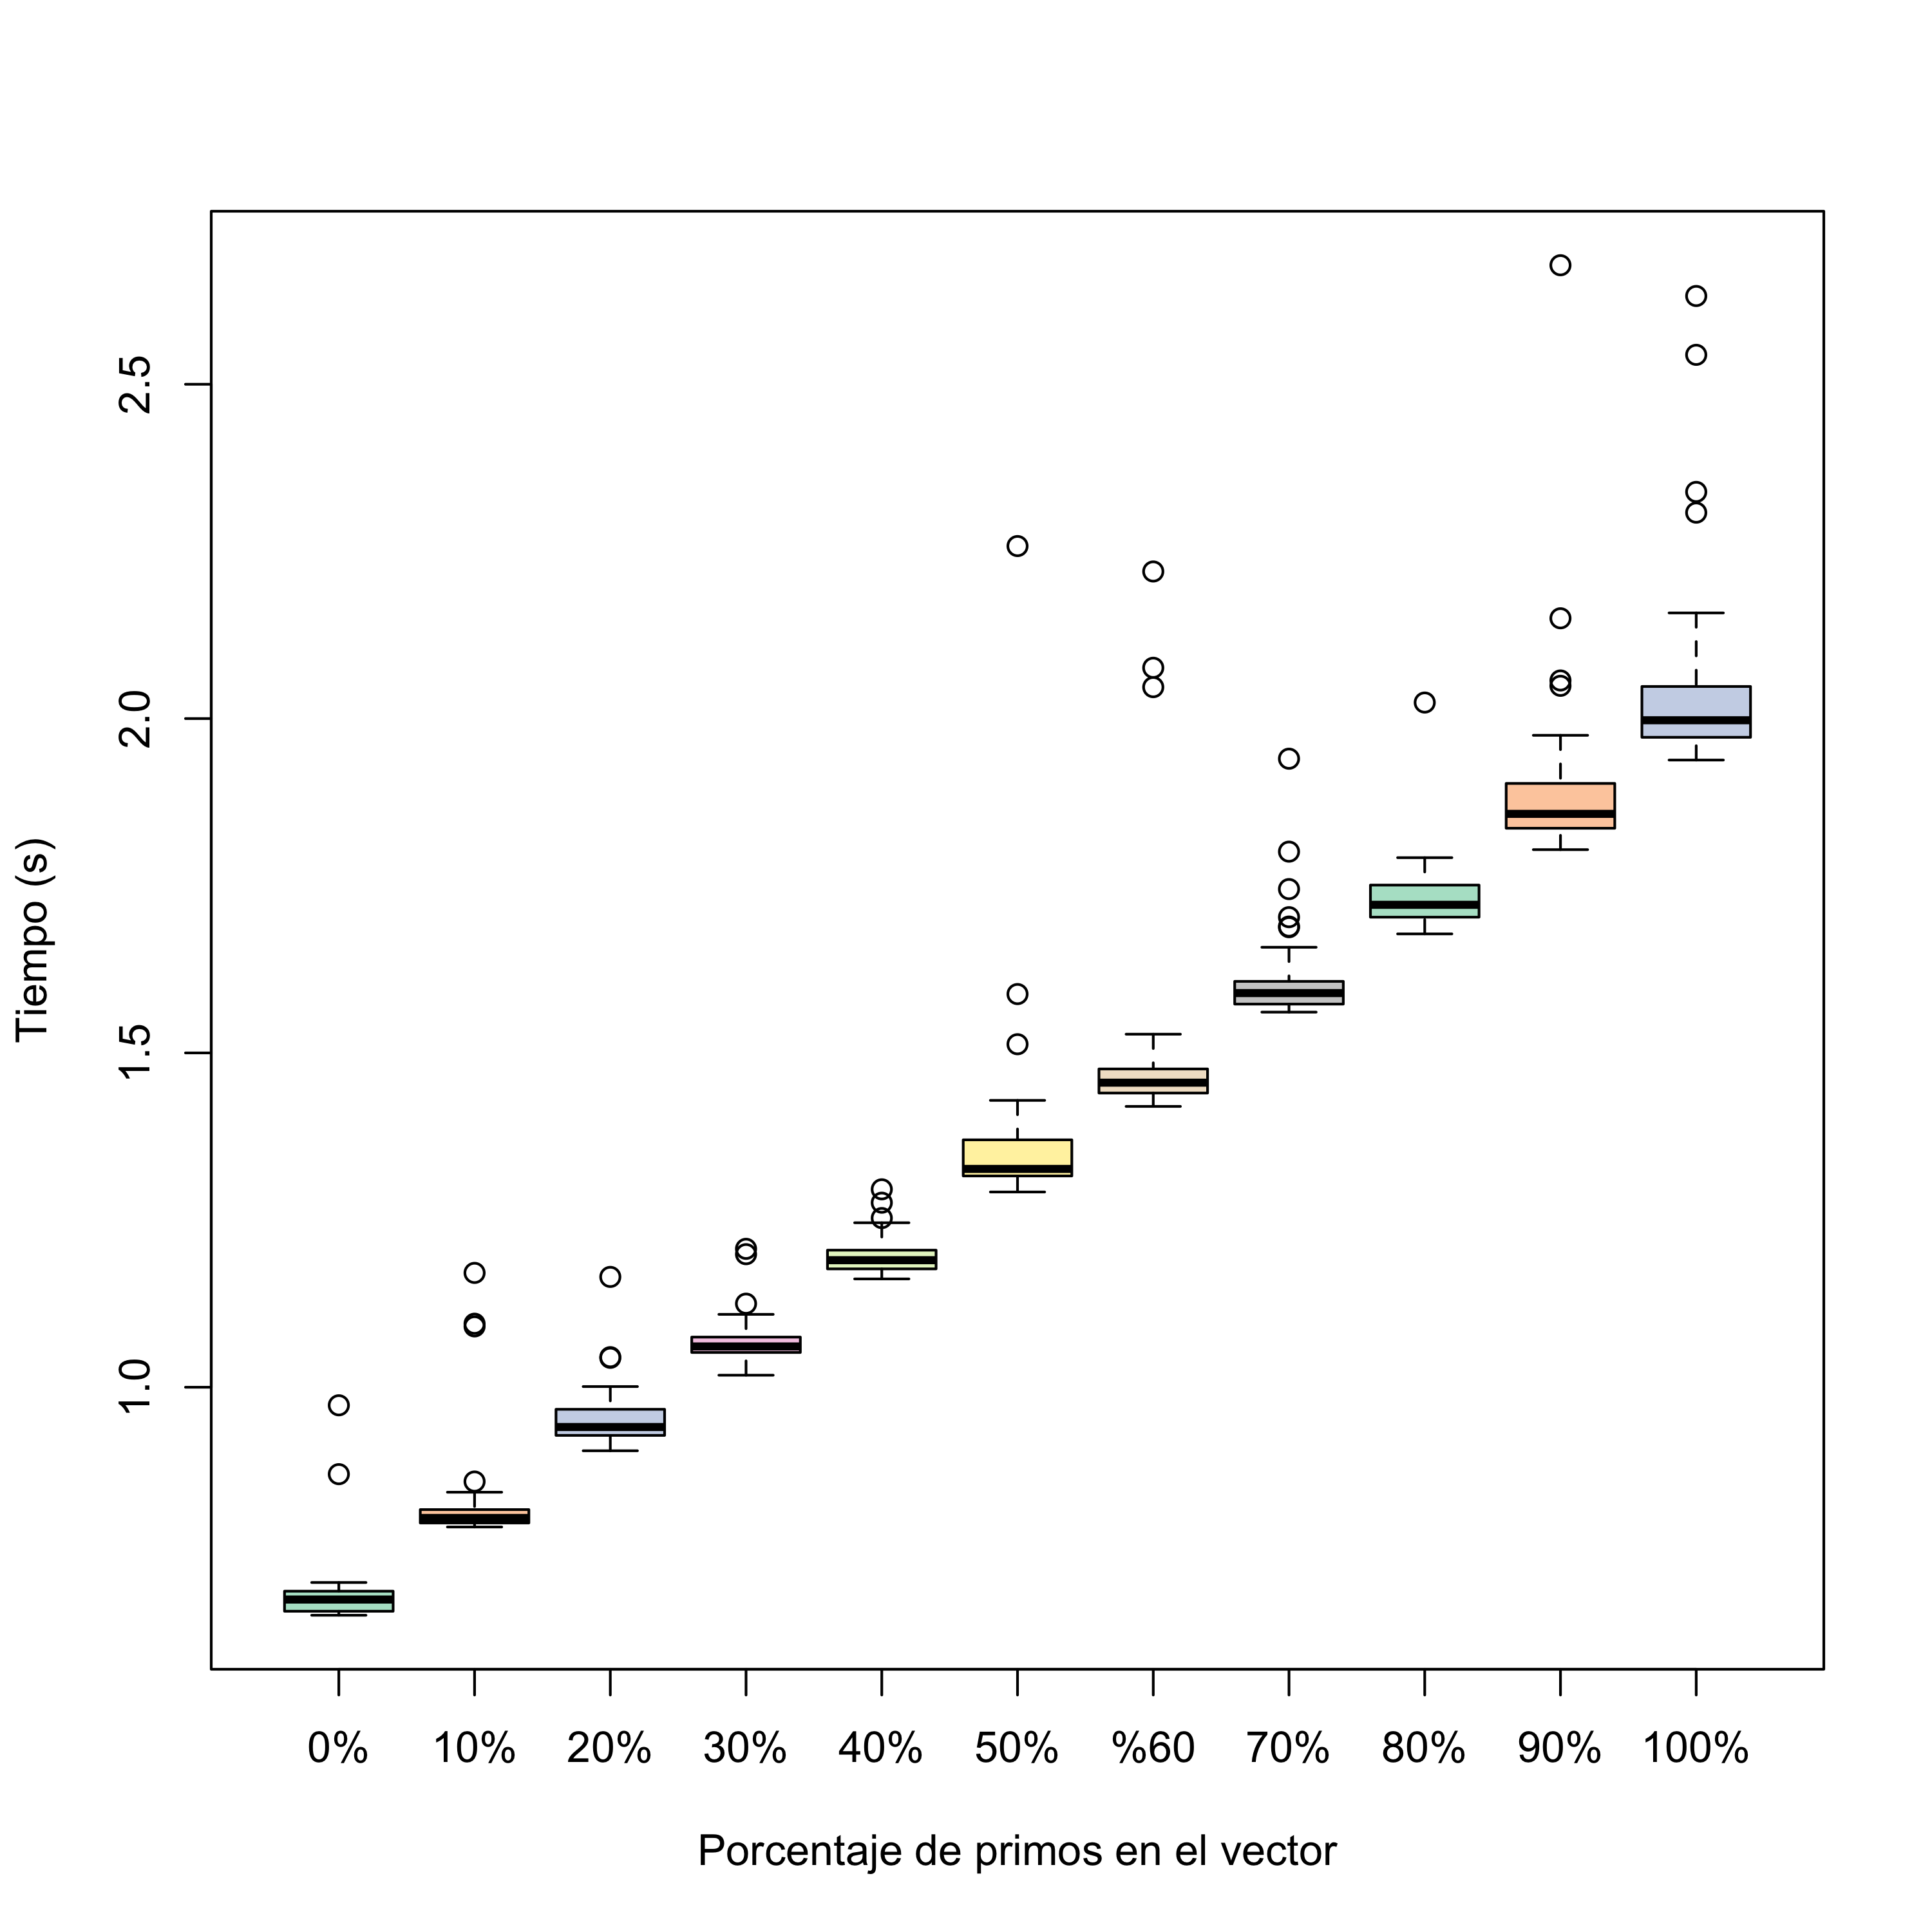
\includegraphics[width=\linewidth]{porcentaje_3.png}
 		\caption{Usando un núcleo.}
 		\label{porcentaje1}
 	\end{subfigure}
 	\caption{Gráfica de cajas variando los núcleos usados en el experimento.}  		
\label{porcentaje}
 \end{figure}
 
 \section{Reto 1}
El primer reto, es modificar la \textit{tarea} para que encuentre todos los divisores de un número $n$. Para ello, se utiliza la función dada en el código \ref{lst:gc2}. En la figura \ref{divisores} tenemos gráficos de caja donde tenemos los tiempos de ejecución de la tarea, variando los núcleos utilizados.
 
En el cuadro \ref{datos3} se tienen los valores $p$ obtenidos al realizar una prueba de Kruskal-Wallis a los datos, para verificar si la cantidad de núcleos utilizados o el orden afectan a los tiempos. En este caso, también lo único que afecta es el orden del vector. 

\begin{lstlisting}[label=lst:gc2,caption=Función para encontrar los divisores de un número., frame = single]
divisores<-function(n) {
    div<-numeric()
    for (i in 1:ceiling(sqrt(n))) {
        if ((n%%  i) == 0) {
            div<-c(div,i)
            div<-c(div,n/i)
        }
    }
    return(sort(unique(div)))
}
\end{lstlisting} 
\begin{table}
\centering
\caption{Valores $p$ obtenidos de la prueba de Kruskal-Wallis en el experimento usando la \textit{tarea} de encontrar los divisores.}
\begin{tabular}{|c|c|}
\hline 
Datos & valor $p$ \\ 
\hline 
Tiempo $\sim$ Núcleo & 0.0018 \\ 
\hline 
Tiempo $\sim$ Orden & 0.6029\\ 
\hline 
\end{tabular} 
\label{datos3}
\end{table} 
 \begin{figure}
 	\centering
 	\begin{subfigure}[b]{0.45\linewidth}
 		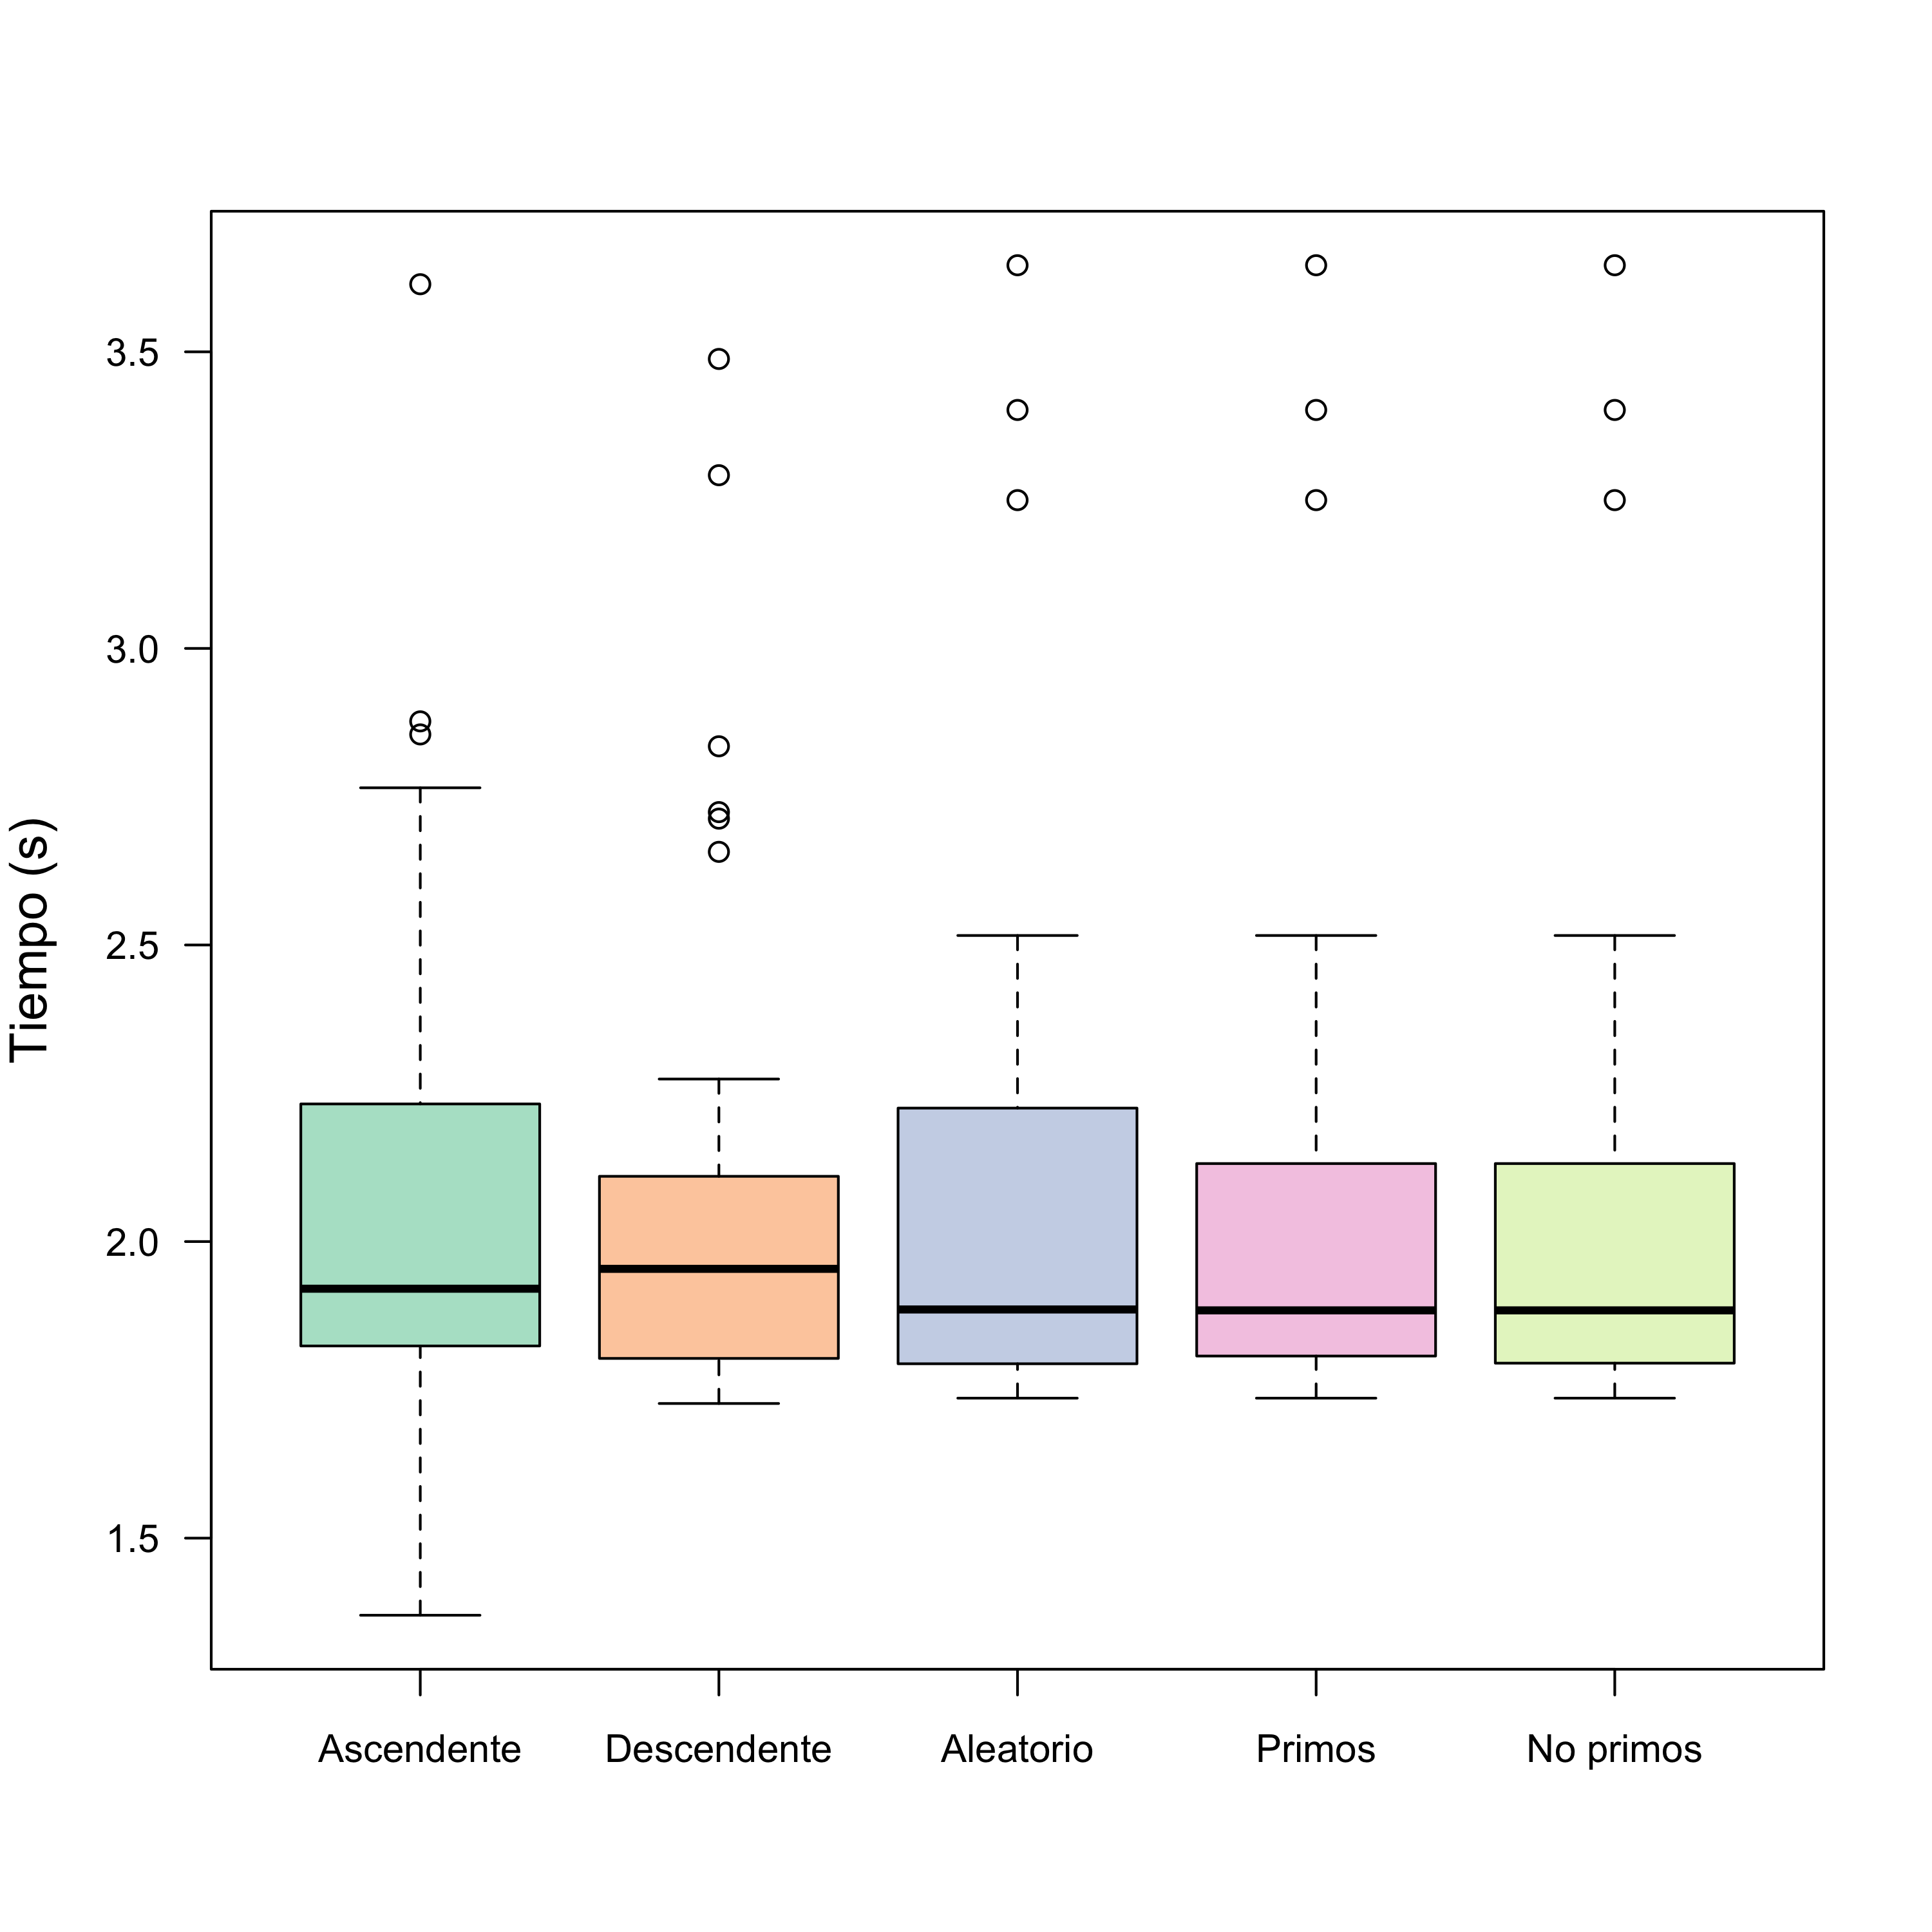
\includegraphics[width=\linewidth]{divisores_1.png}
 		 \caption{Usando tres núcleos.}
 		\label{divisores3}
 	\end{subfigure}
 	\begin{subfigure}[b]{0.45\linewidth}
 		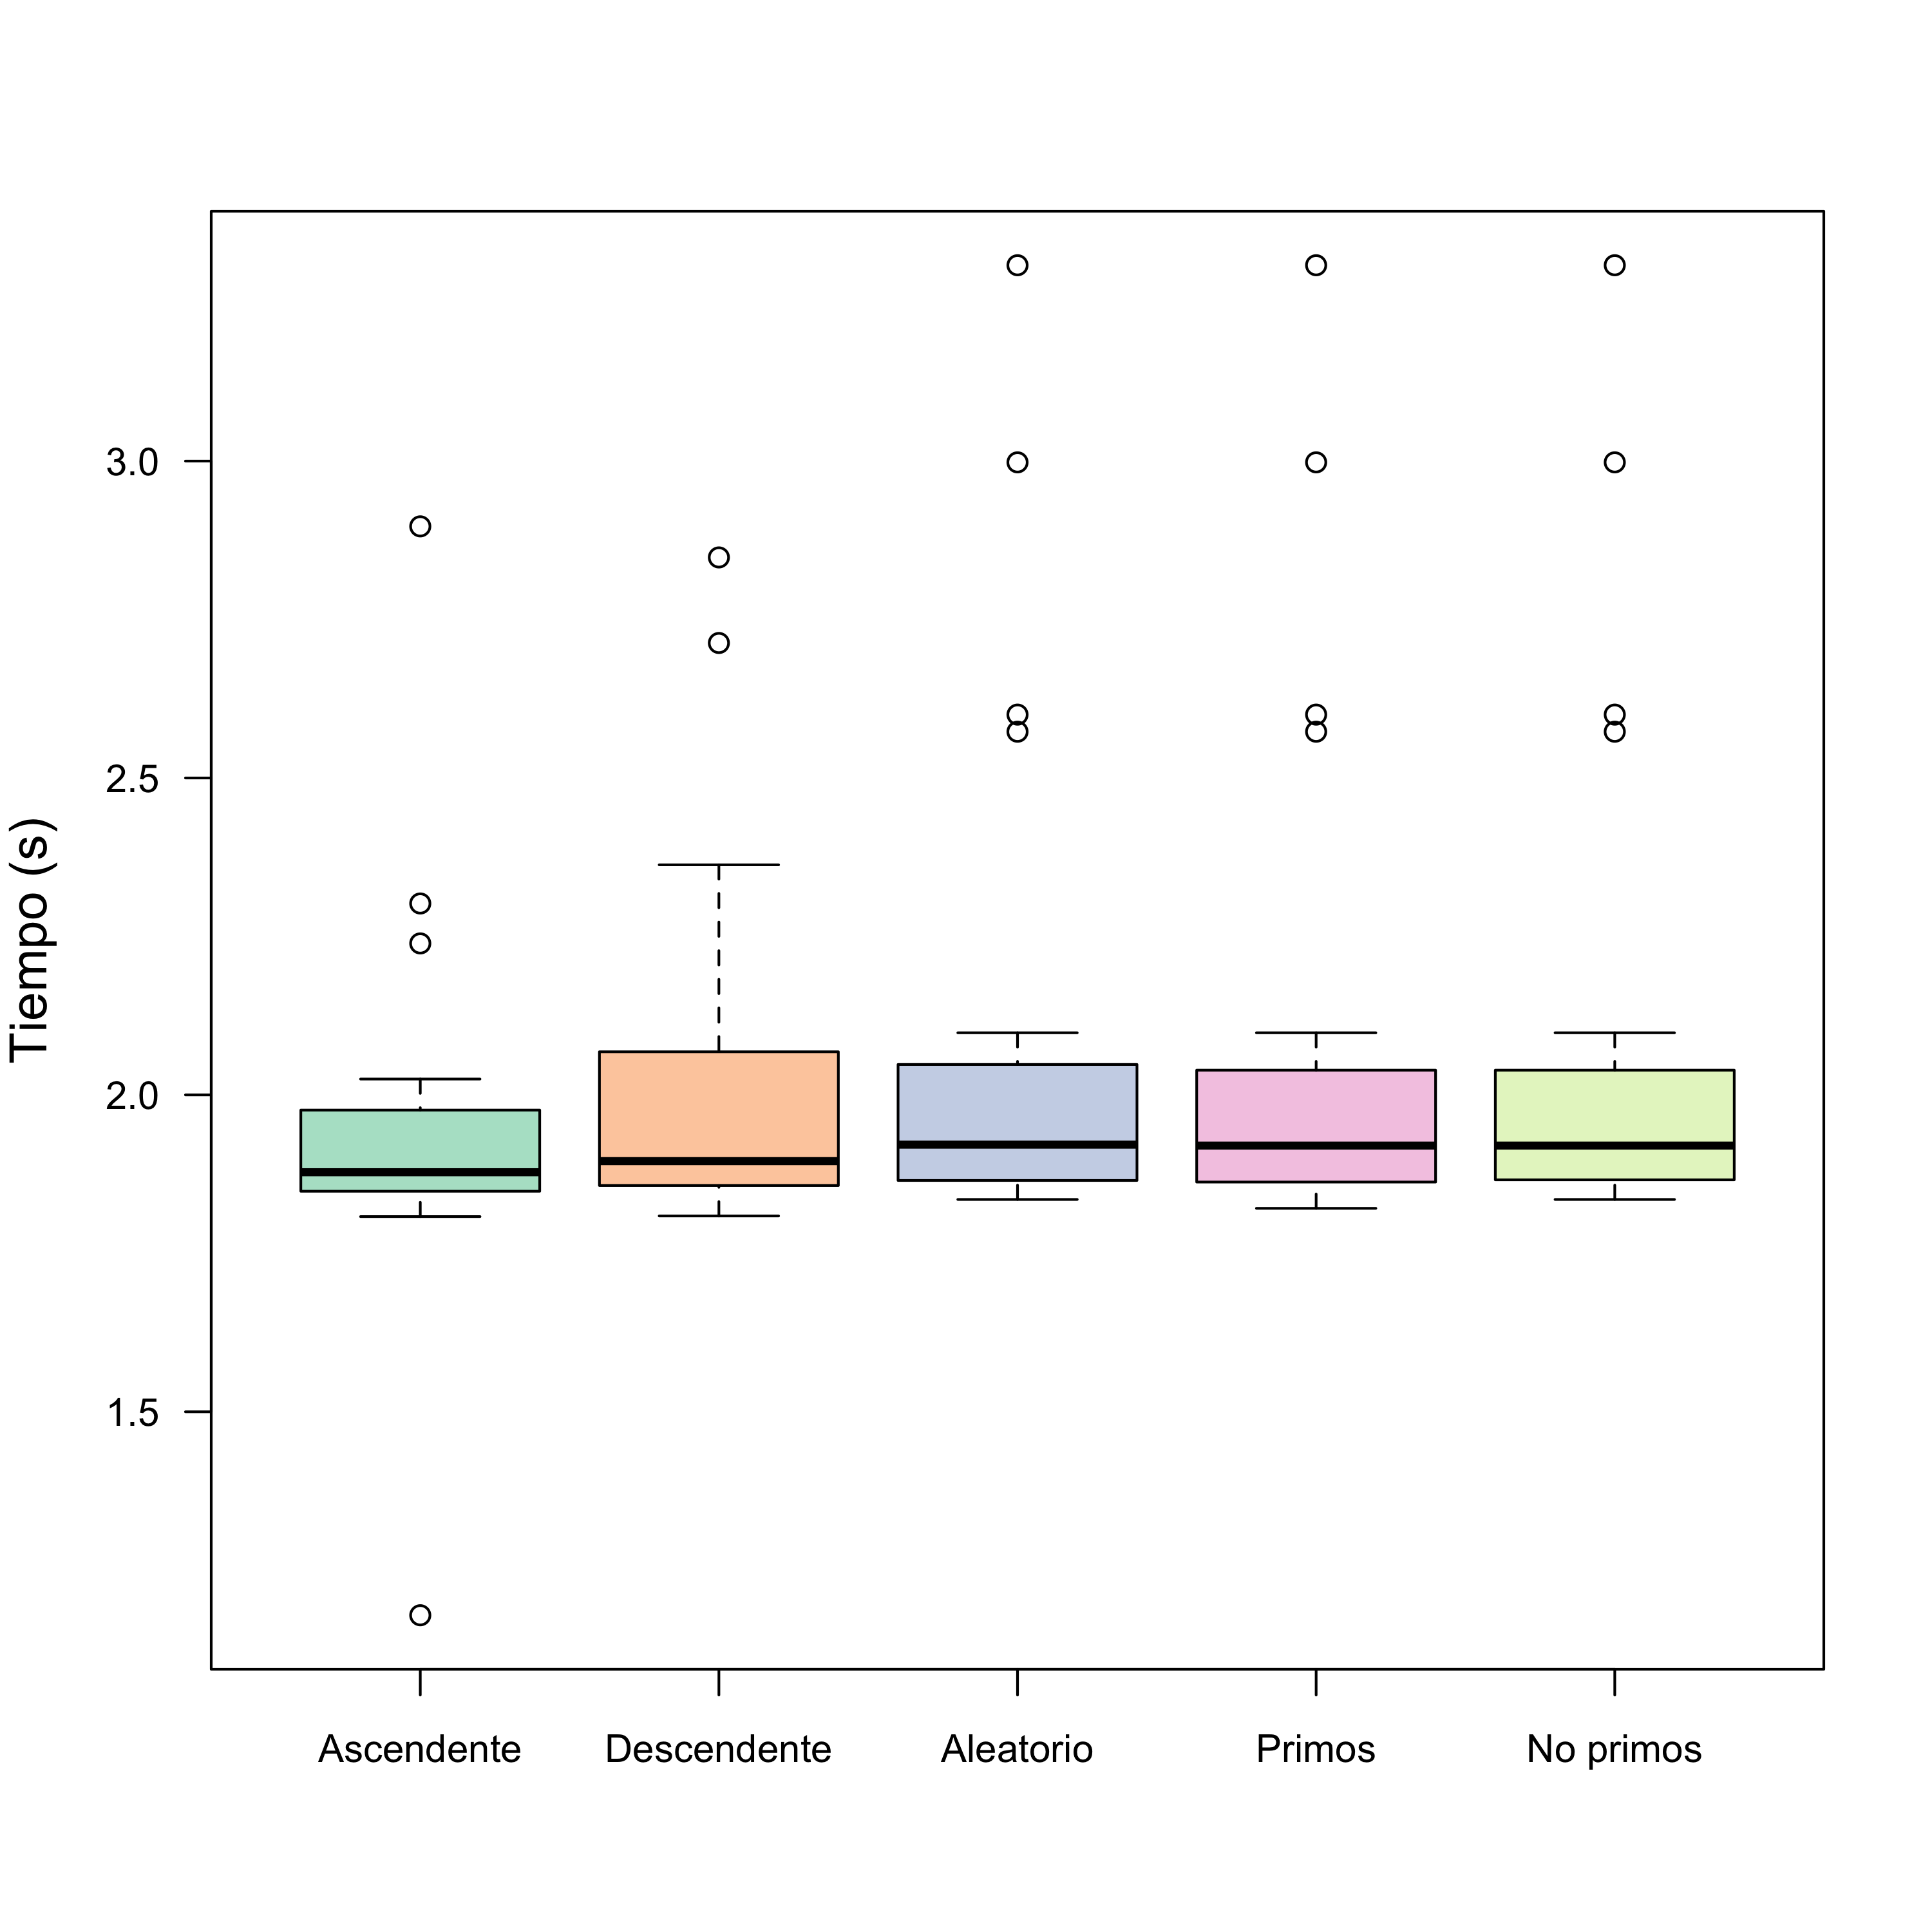
\includegraphics[width=\linewidth]{divisores_2.png}
 		 \caption{Usando dos núcleos.}
 		\label{divisores2}
 	\end{subfigure}
 	\begin{subfigure}[b]{0.45\linewidth}
 		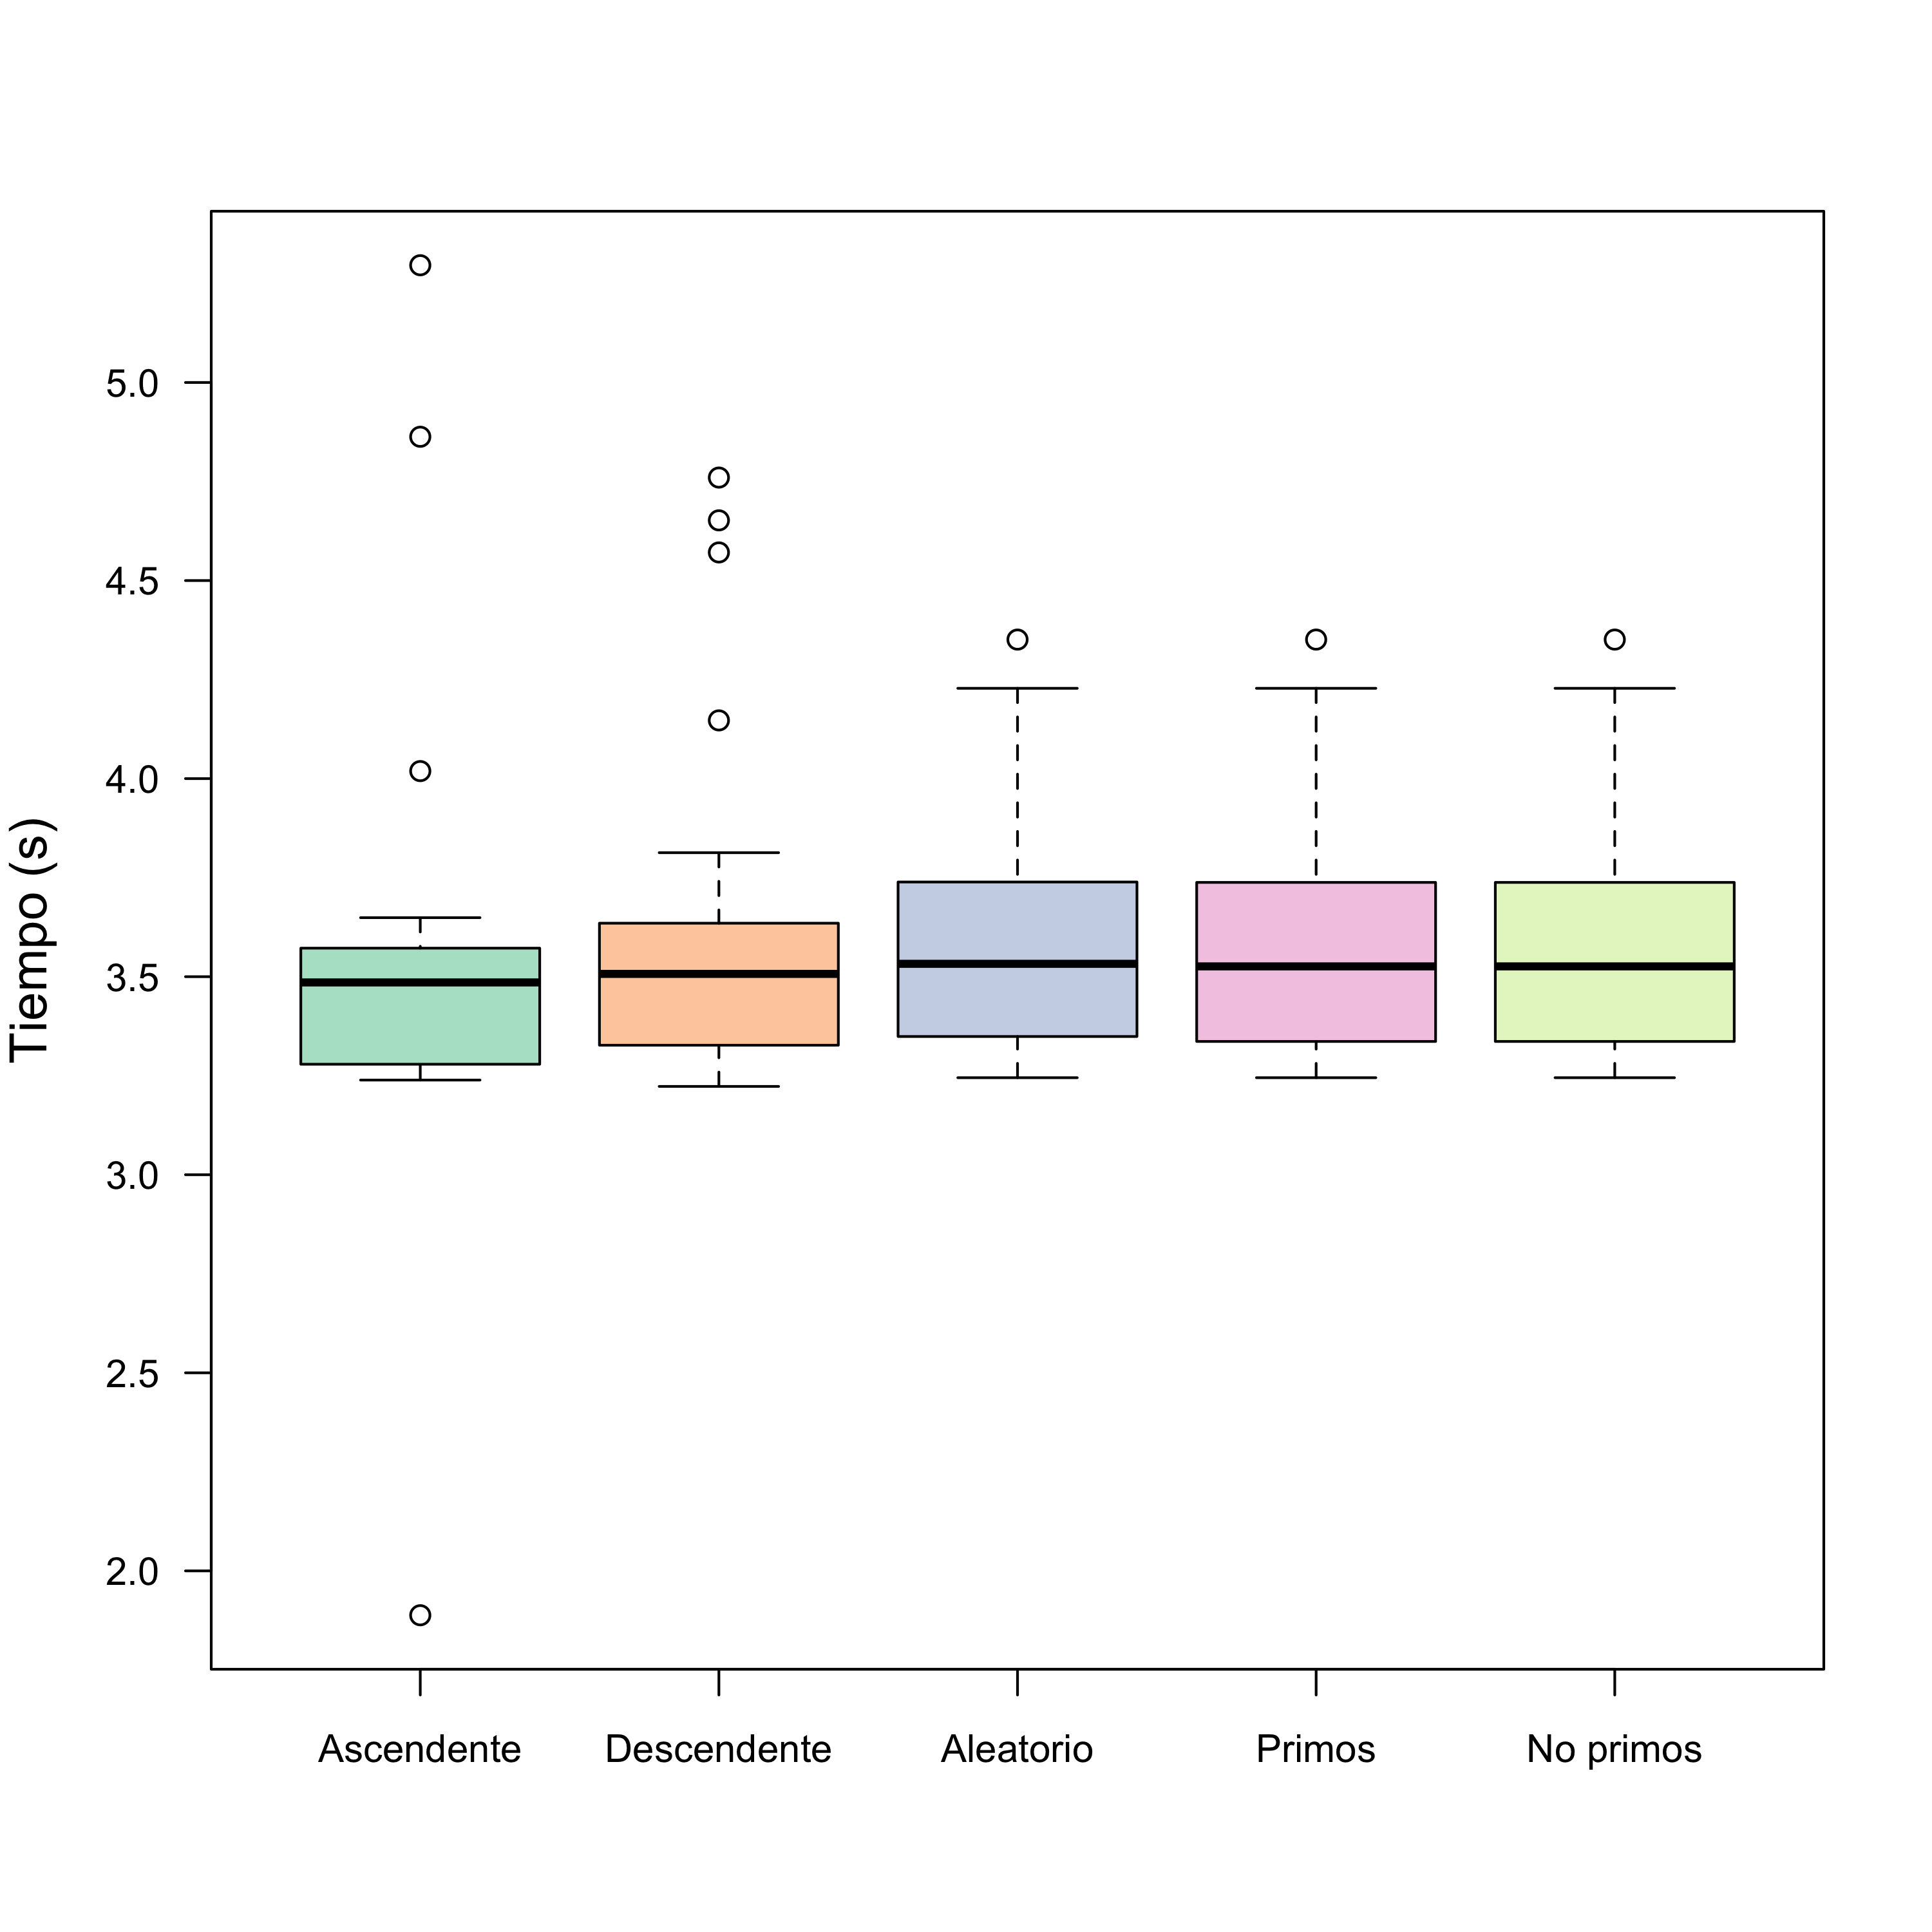
\includegraphics[width=\linewidth]{divisores_3.png}
 		\caption{Usando un núcleo.}
 		\label{divisores1}
 	\end{subfigure}
 	\caption{Gráfica de cajas variando los núcleos usados en el experimento.}  		
\label{divisores}
 \end{figure}
 \section{Reto 2}
En el segundo reto, se modifica la \textit{tarea} para factorizar en primos el número $n$, en este caso se utiliza la función dada en el código \ref{lst:gc3}. En la figura \ref{factorizacion} se tienen los gráficos de caja con los tiempos de ejecución variando los núcleos y en el cuadro \ref{datos4} se tiene los valores $p$ que se obtienen al realizar una prueba de Kruskal-Wallis. Nuevamente, en este caso lo que afecta es el orden del vector.

En ninguno de los dos retos, cambiamos las conclusiones obtenidas en el primer experimento.

\begin{lstlisting}[label=lst:gc3,caption=Función para factorizar en primos un número., frame = single]
fact_primos<-function(n) {
    div<-numeric()
    while(n%%  2 == 0) {
    div<-c(div,2)
    n = n/2
    }
    for(i in seq(3, max(3, ceiling(sqrt(n))), 2)) {
        while(n%%  i==0) {
            div<-c(div,i)
            n=n/i
        }
    }
    if(n>2){ div<-c(div,n) }
    return(table(div))
}
\end{lstlisting} 
\begin{table}
\centering
\caption{Valores $p$ obtenidos de la prueba de Kruskal-Wallis en el experimento usando la \textit{tarea} de factorizar en primos.}
\begin{tabular}{|c|c|}
\hline 
Datos & valor $p$ \\ 
\hline 
Tiempo $\sim$ Núcleo & 0.0025 \\ 
\hline 
Tiempo $\sim$ Orden & 0.5234\\ 
\hline 
\end{tabular} 
\label{datos4}
\end{table} 
 \begin{figure}
 	\centering
 	\begin{subfigure}[b]{0.45\linewidth}
 		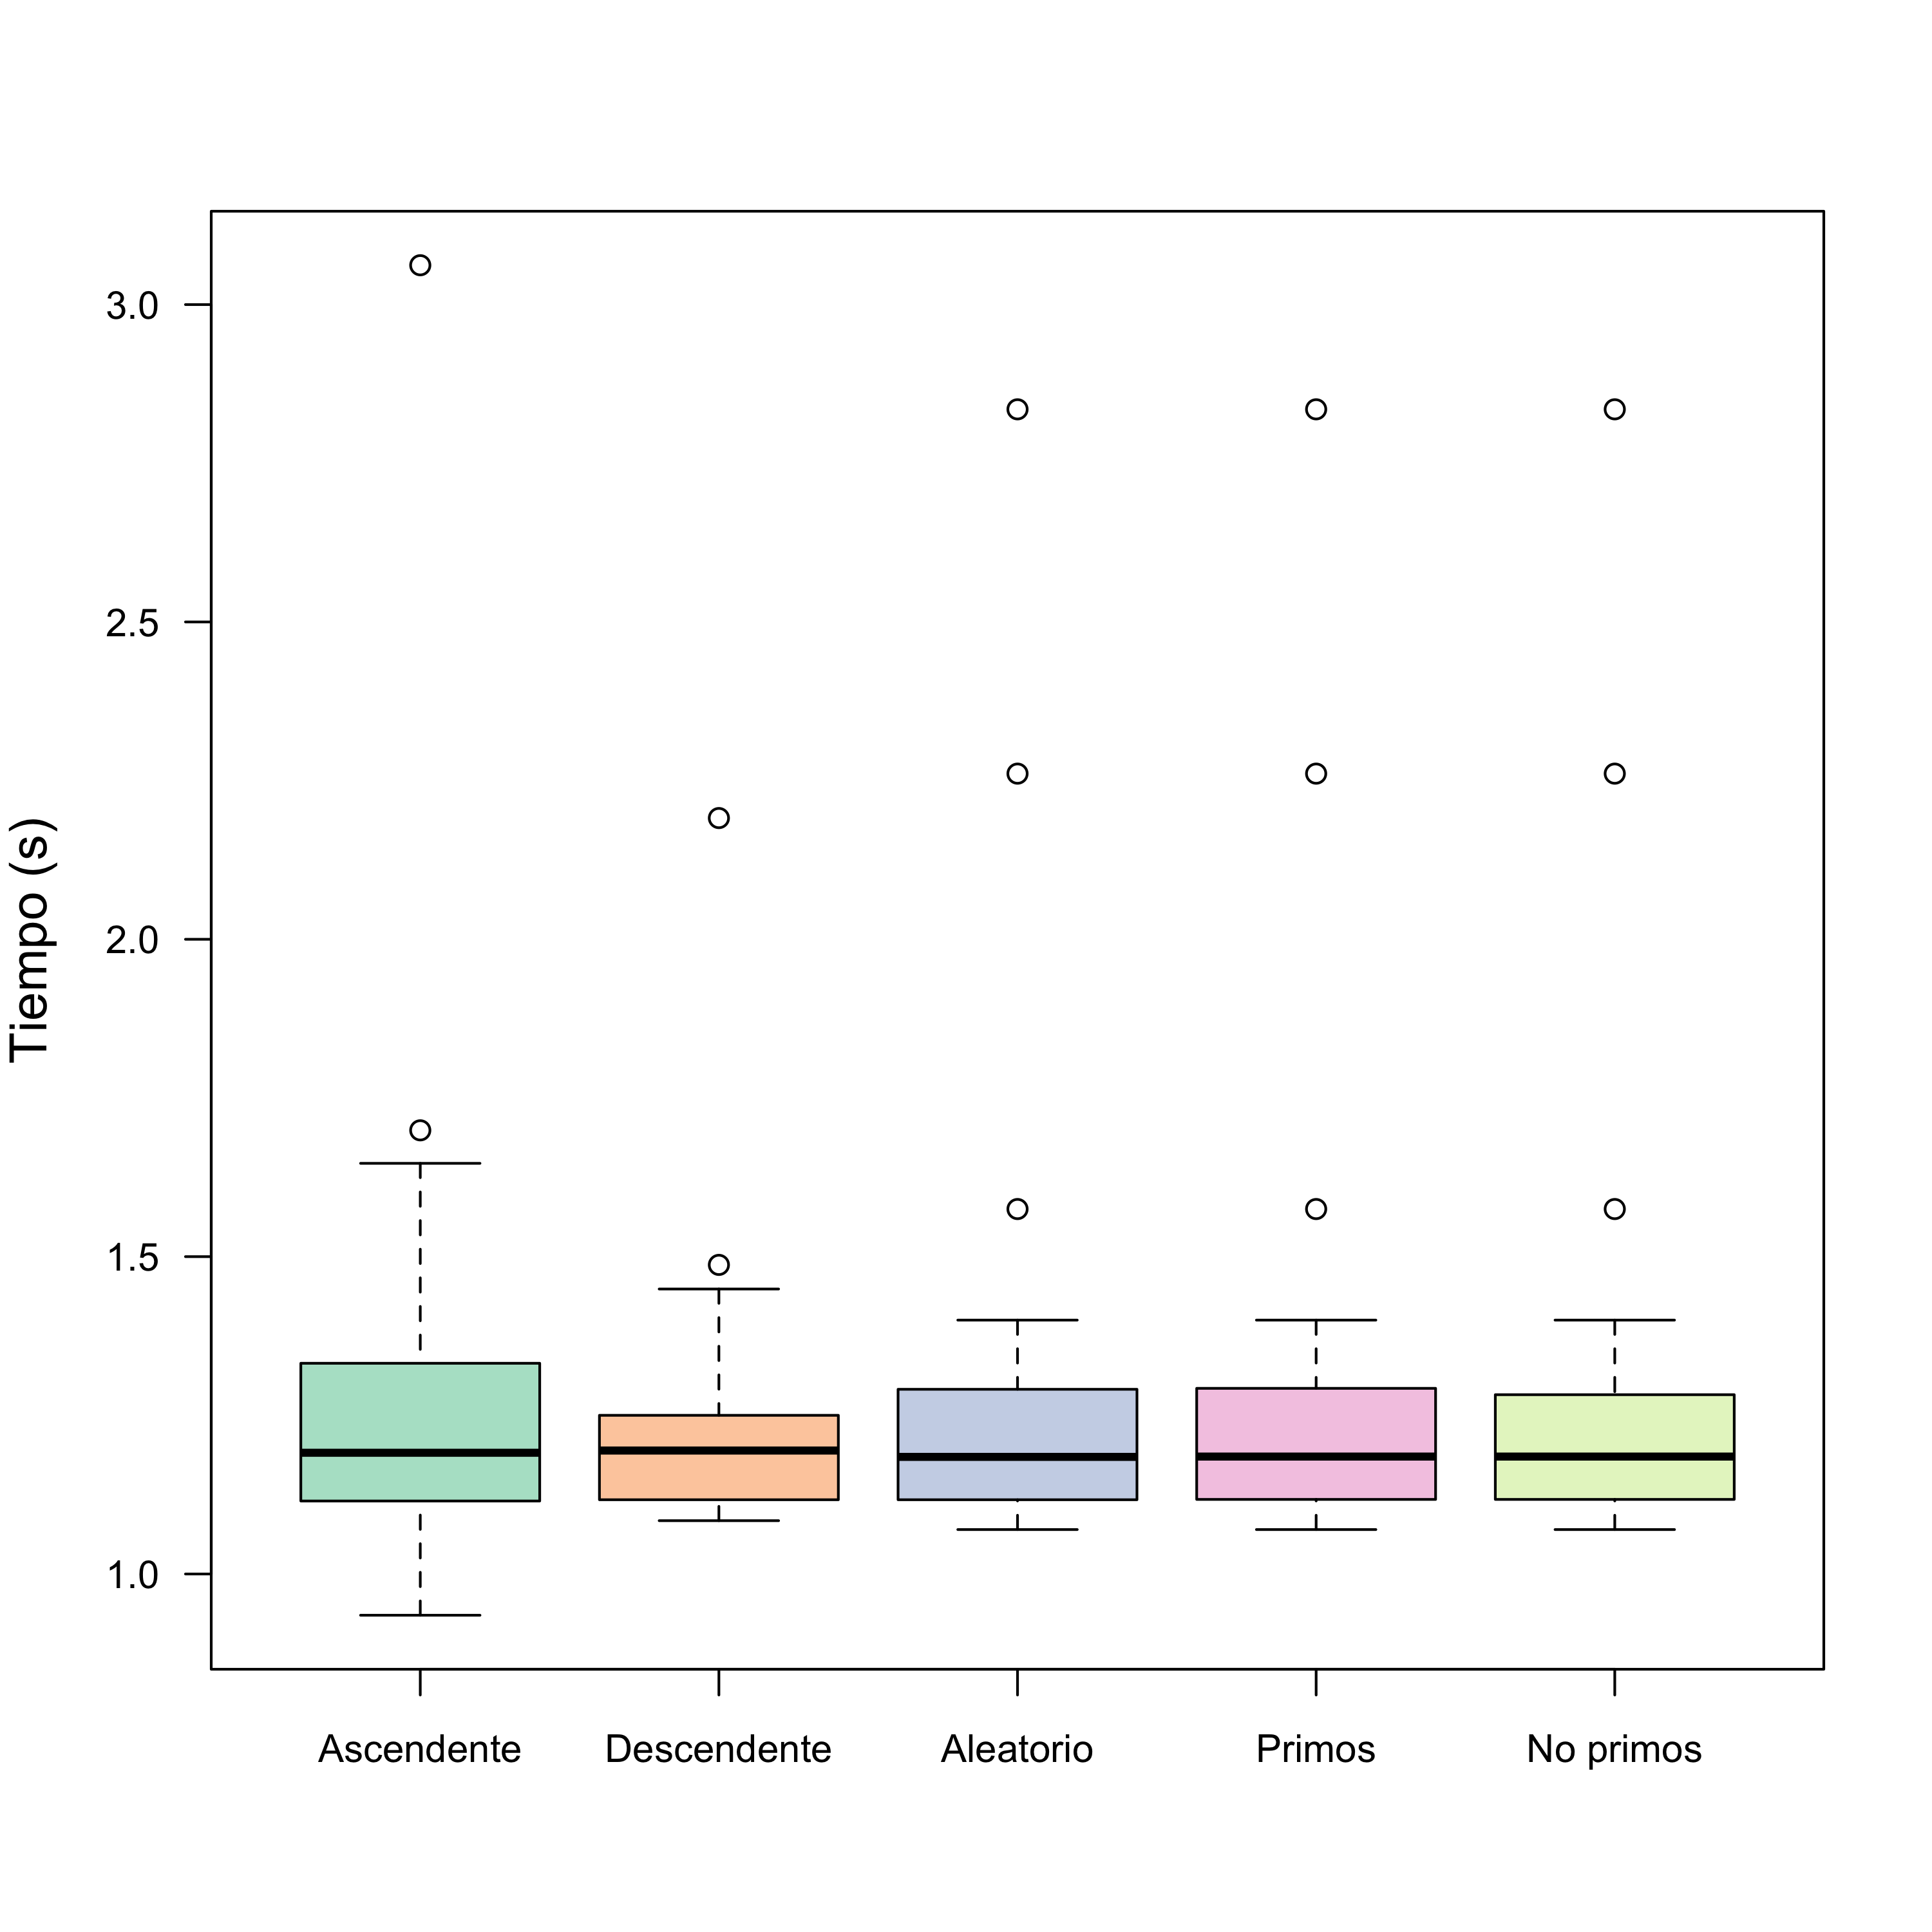
\includegraphics[width=\linewidth]{factorizacion_1.png}
 		 \caption{Usando tres núcleos.}
 		\label{factorizacion3}
 	\end{subfigure}
 	\begin{subfigure}[b]{0.45\linewidth}
 		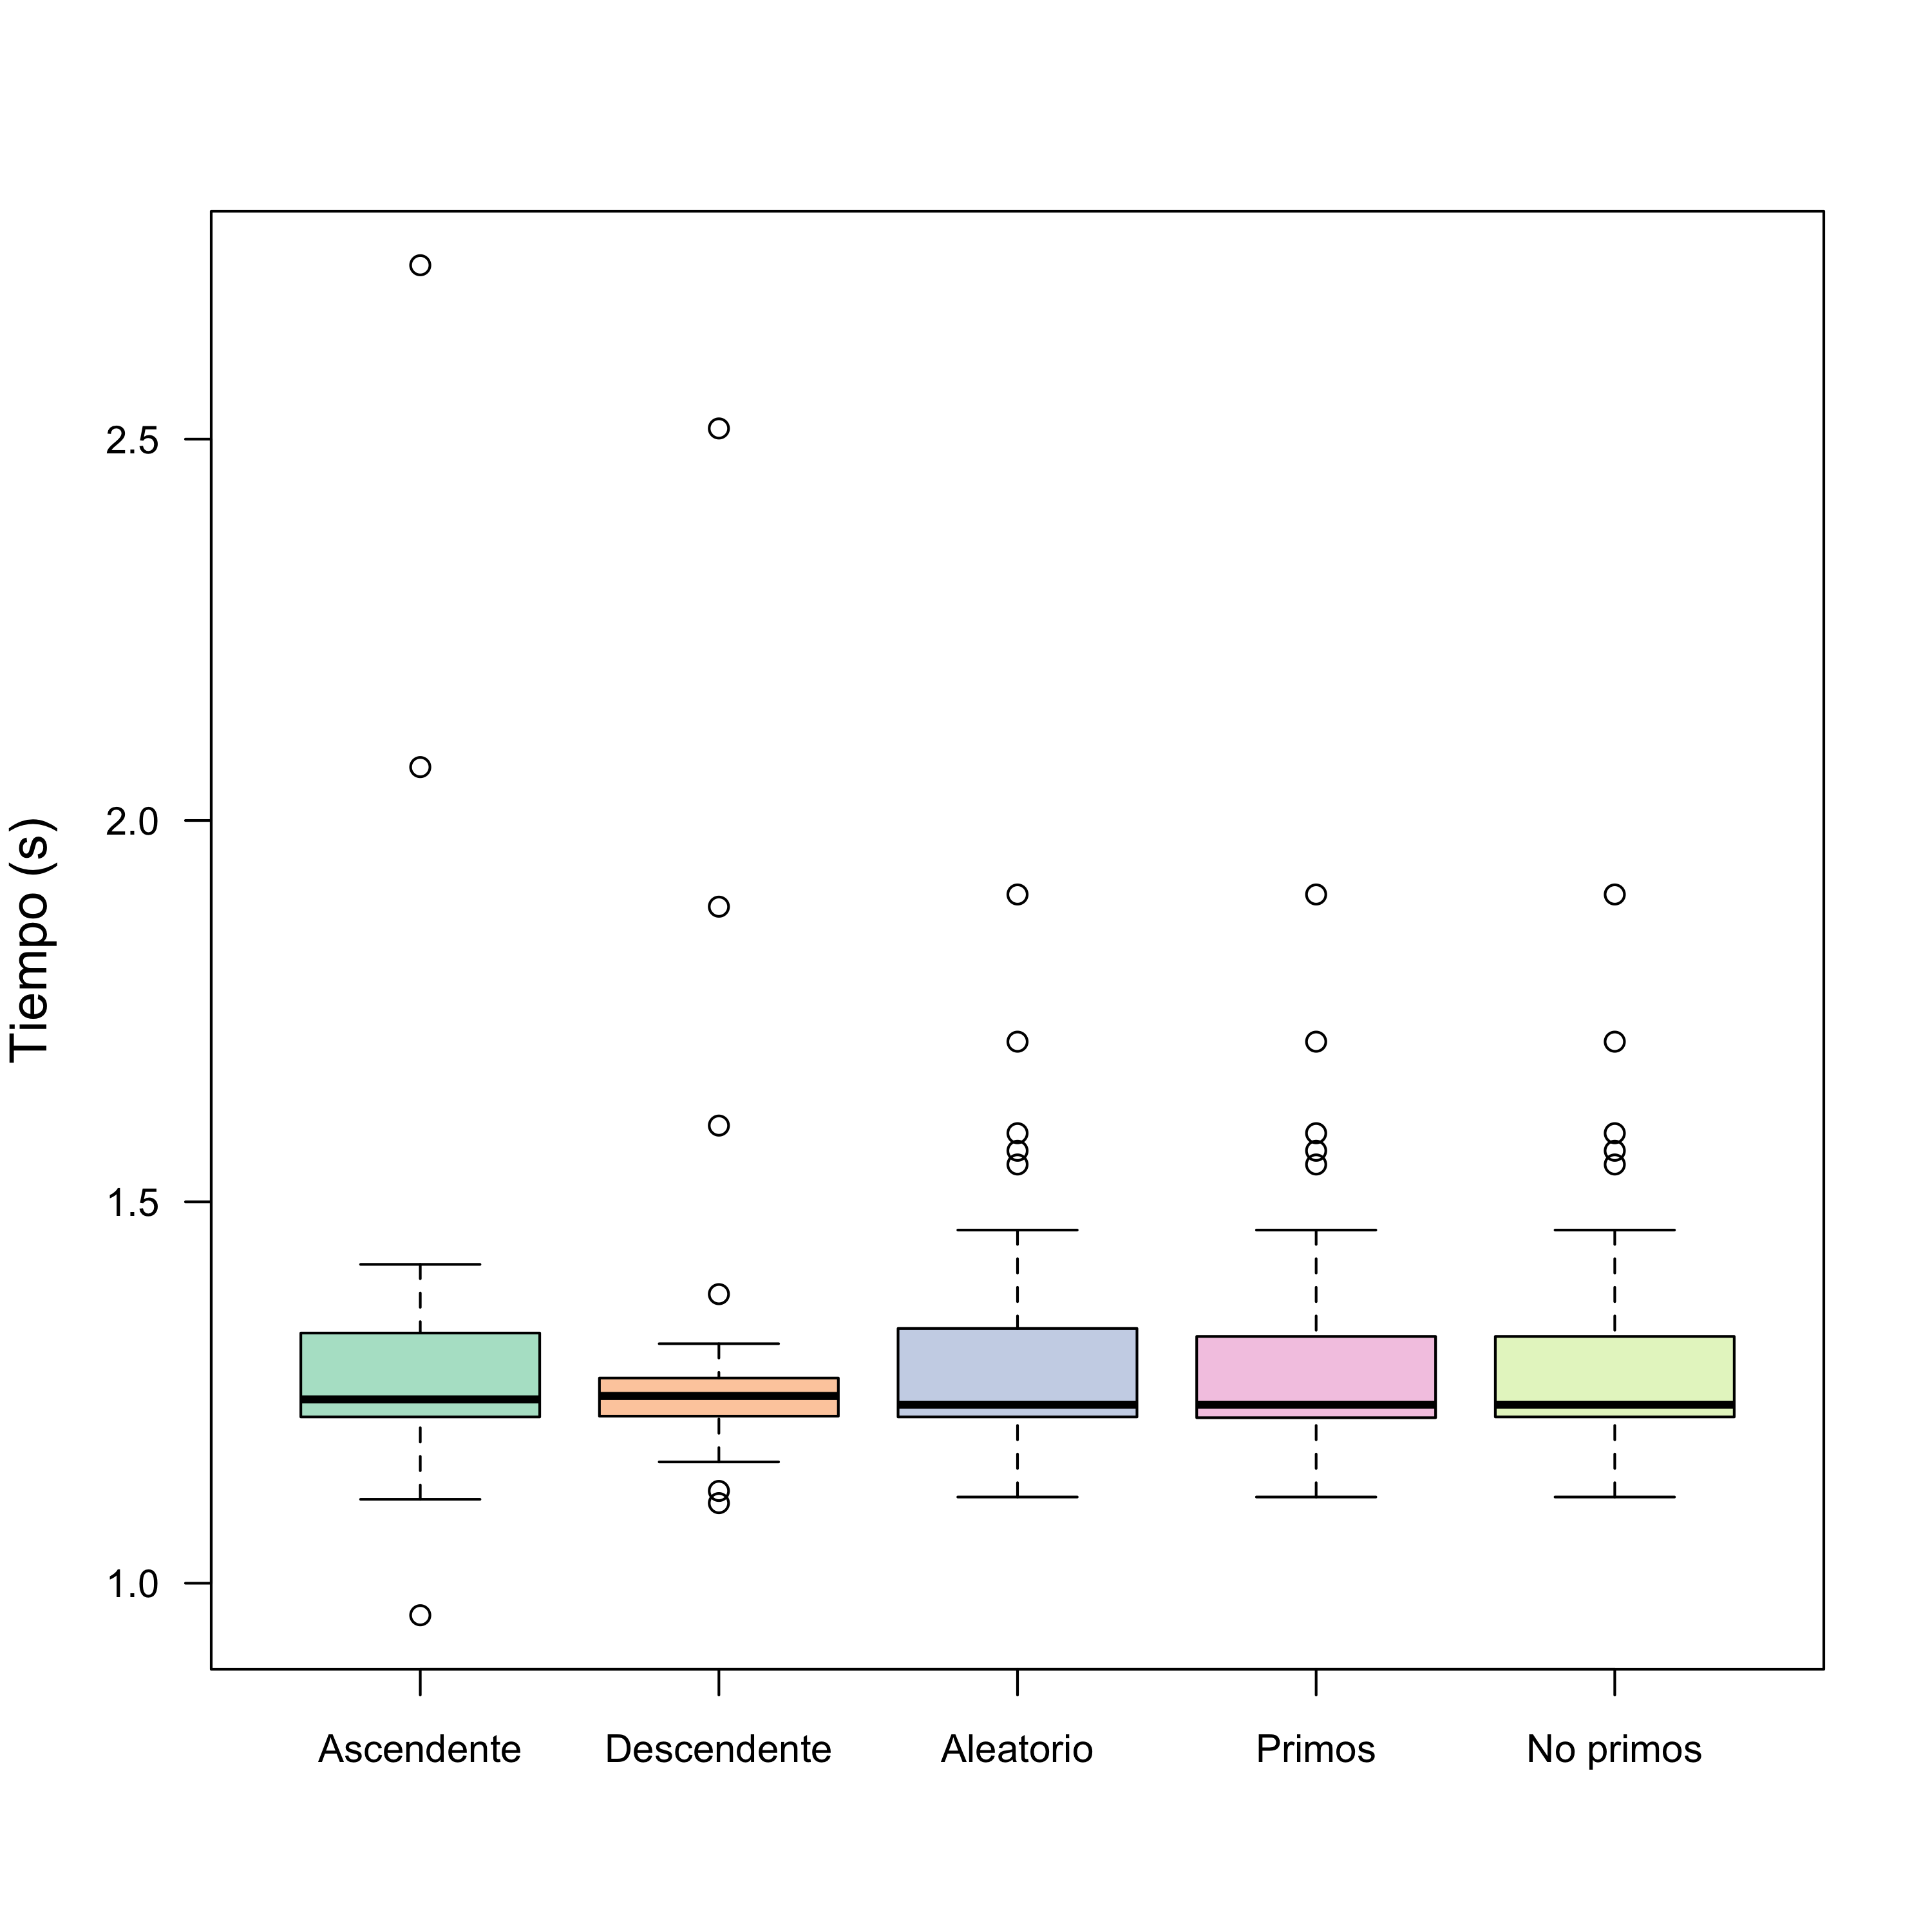
\includegraphics[width=\linewidth]{factorizacion_2.png}
 		 \caption{Usando dos núcleos.}
 		\label{factorizacion2}
 	\end{subfigure}
 	\begin{subfigure}[b]{0.45\linewidth}
 		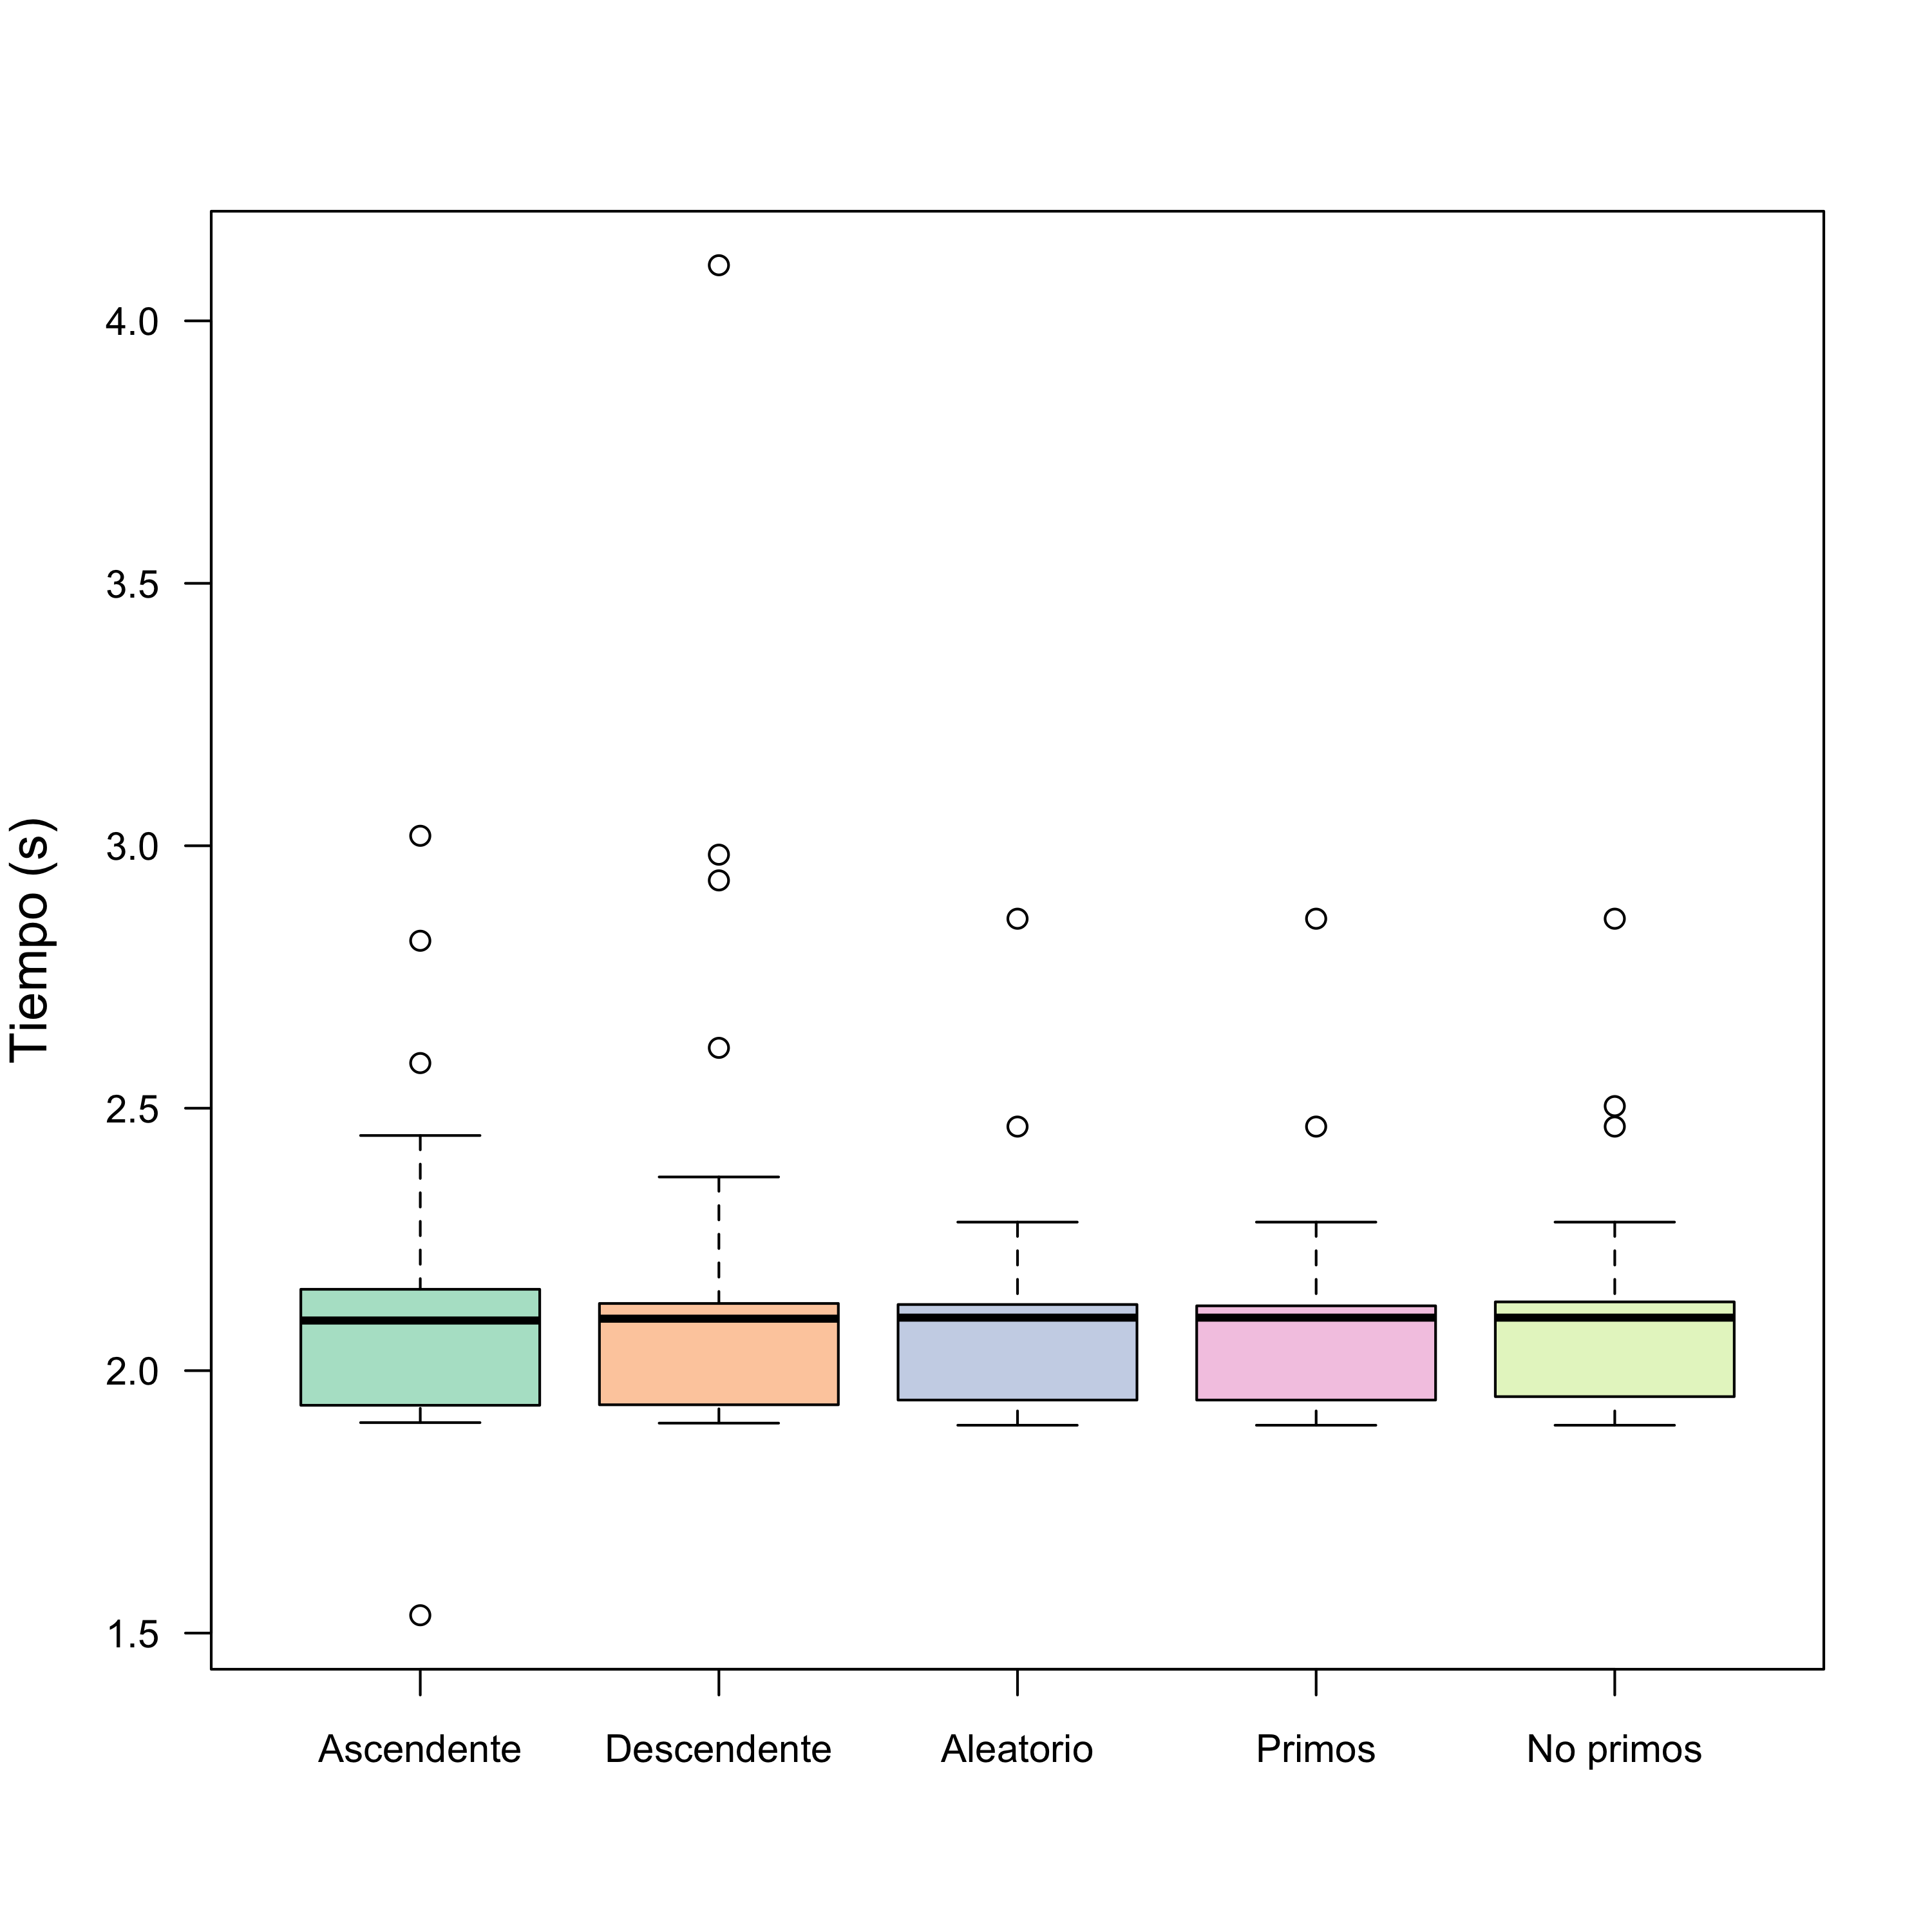
\includegraphics[width=\linewidth]{factorizacion_3.png}
 		\caption{Usando un núcleo.}
 		\label{factorizacion1}
 	\end{subfigure}
 	\caption{Gráfica de cajas variando los núcleos usados en el experimento.}  		
\label{factorizacion}
 \end{figure}
\bibliographystyle{plain} 
\bibliography{Referencias}
\end{document}